\batchmode
\nonstopmode
\documentclass[oneside]{article}
\n
% Packages required by doxygen
\usepackage{calc}
\usepackage{doxygen}
\usepackage{listings}
\usepackage{graphicx}
\usepackage[utf8]{inputenc}
\usepackage{makeidx}
\usepackage{multicol}
\usepackage{multirow}
\usepackage{textcomp}
\usepackage{amsmath}
\usepackage[table]{xcolor}
\usepackage{indentfirst}

% Font selection
\usepackage[T1]{fontenc}
\usepackage{mathptmx}
\usepackage[scaled=.90]{helvet}
\usepackage{courier}
\usepackage{amssymb}
\usepackage{sectsty}
\renewcommand{\familydefault}{\sfdefault}
\allsectionsfont{%
  \fontseries{bc}\selectfont%
  \color{darkgray}%
}
\renewcommand{\DoxyLabelFont}{%
  \fontseries{bc}\selectfont%
  \color{darkgray}%
}

% Page & text layout
\usepackage{geometry}
\geometry{%
  a4paper,%
  top=2.5cm,%
  bottom=2.5cm,%
  left=2.5cm,%
  right=2.5cm%
}
\tolerance=750
\hfuzz=15pt
\hbadness=750
\setlength{\emergencystretch}{15pt}
\setlength{\parindent}{0cm}
\setlength{\parskip}{0.2cm}
\makeatletter
\renewcommand{\paragraph}{%
  \@startsection{paragraph}{4}{0ex}{-1.0ex}{1.0ex}{%
\normalfont\normalsize\bfseries\SS@parafont%
  }%
}
\renewcommand{\subparagraph}{%
  \@startsection{subparagraph}{5}{0ex}{-1.0ex}{1.0ex}{%
\normalfont\normalsize\bfseries\SS@subparafont%
  }%
}
\makeatother

% Used by @code ... @endcode
\renewenvironment{DoxyCode}{%
  \par
  \normalsize
  \begin{alltt}%
}{%
  \end{alltt}%
  \normalsize%
}
% Headers & footers
\usepackage{fancyhdr}
\pagestyle{fancyplain}
\fancyhead[LE]{\fancyplain{}{\bfseries\thepage}}
\fancyhead[CE]{\fancyplain{}{}}
\fancyhead[RE]{\fancyplain{}{\bfseries\leftmark}}
\fancyhead[LO]{\fancyplain{}{\bfseries\rightmark}}
\fancyhead[CO]{\fancyplain{}{}}
\fancyhead[RO]{\fancyplain{}{\bfseries\thepage}}
\fancyfoot[LE]{\fancyplain{}{}}
\fancyfoot[CE]{\fancyplain{}{}}
\fancyfoot[RE]{\fancyplain{}{\bfseries\scriptsize PythonOCC User Guide - STEP processor  }}% : STEP processor  }}
\fancyfoot[LO]{\fancyplain{}{\bfseries\scriptsize PythonOCC User Guide - STEP processor  }}% : STEP processor  }
\fancyfoot[CO]{\fancyplain{}{}}
\fancyfoot[RO]{\fancyplain{}{}}
\renewcommand{\footrulewidth}{0.4pt}
\renewcommand{\sectionmark}[1]{%
  \markright{\thesection\ #1}%
}

% Indices & bibliography
\usepackage{natbib}
\usepackage[titles]{tocloft}
\renewcommand{\cftsecleader}{\cftdotfill{\cftdotsep}}
\setcounter{tocdepth}{3}
\setcounter{secnumdepth}{5}
\makeindex

% Hyperlinks (required, but should be loaded last)
\usepackage{ifpdf}
\ifpdf
  \usepackage[pdftex,pagebackref=true]{hyperref}
\else
  \usepackage[ps2pdf,pagebackref=true]{hyperref}
\fi
\hypersetup{%
  colorlinks=true,%
  linkcolor=black,%
  citecolor=black,%
  urlcolor=blue,%
  unicode%
}

% Custom commands
\newcommand{\clearemptydoublepage}{%
  \newpage{\pagestyle{empty}\cleardoublepage}%
}
\n


%===== C O N T E N T S =====\n
\begin{document}
% Titlepage & ToC
\hypersetup{pageanchor=false}
\pagenumbering{roman}
\begin{titlepage}
\vspace*{7cm}
\begin{center}%
\includegraphics[width=150px, height=150px]{../../../dox/resources/logo_pythonocc.png}\\
\vspace*{1cm}
{\Large PythonOCC 0.18.2 Documentation}\\
{\Large STEP processor  }\\
\vspace*{1cm}
{\small Thomas Paviot - \email{tpaviot@gmail.com}}\\
{\small originally written by the OpenCASCADE company}\\

\vspace*{1cm}
{\small Document version 0 - \today}\
\end{center}
\end{titlepage}
\clearpage
\pagenumbering{roman}
\tableofcontents
\newpage
\pagenumbering{arabic}
\hypersetup{pageanchor=true}

\let\stdsection\section
  \renewcommand\section{\pagebreak\stdsection}
\hypertarget{occt_user_guides__step}{}
\hypertarget{occt_user_guides__step_occt_step_1}{}\section{Introduction}\label{occt_user_guides__step_occt_step_1}
S\+T\+EP is more and more widely used to exchange data between various software, involved in C\+AD, P\+DM, Analysis, etc... S\+T\+EP is far more than an \char`\"{}exchange standard\char`\"{} \+: it provides a technology and a set of methodologies to describe the data to exchange in a modular and upgradeable way. Regarding O\+C\+CT, this mostly applies to C\+AD data but it is not a limitation, other kinds of data for specific applications can be addressed too.


\begin{DoxyImage}
\begin{center}
 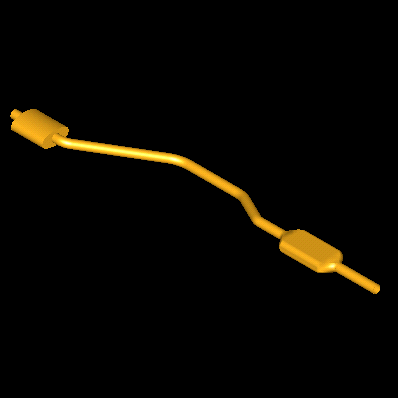
\includegraphics[width=\textwidth,height=\textheight/2,keepaspectratio=true]{step_image002.png}
\end{center}
\caption{Image imported from S\+T\+EP}
\end{DoxyImage}


Open Cascade allows its users to employ S\+T\+EP in the following domains\+:
\begin{DoxyItemize}
\item Exchange of data for technical applications, following the state-\/of-\/the-\/art definitions and rules;
\item Extension of case coverage, according to specific needs or to the evolution of general business uses;
\item Expertise in data architecture of an application, to get experience from S\+T\+EP definitions and make easier the mapping to them, for a better interoperability with outer world.
\end{DoxyItemize}

This manual is intended to provide technical documentation on the Open C\+A\+S\+C\+A\+DE Technology ({\bfseries O\+C\+CT}) S\+T\+EP processor and to help Open C\+A\+S\+C\+A\+DE Technology users with the use of the S\+T\+EP processor (to read and write S\+T\+EP files).

Only geometrical, topological S\+T\+EP entities (shapes) and assembly structures are translated by the basic translator described in sections 2 to 6. Data that cannot be translated on this level are also loaded from a S\+T\+EP file and can be translated later. X\+DE S\+T\+EP translator (see section 7 \href{#occt_step_7}{\tt Reading from and writing to X\+DE}) translates names, colors, layers, validation properties and other data associated with shapes and assemblies into X\+DE document.

File translation is performed in the programming mode, via C++ calls.

Shape Healing toolkit provides tools to heal various problems, which may be encountered in translated shapes, and to make them valid in Open C\+A\+S\+C\+A\+DE. The Shape Healing is smoothly connected to S\+T\+EP translator using the same A\+PI, only the names of A\+PI packages change.

For testing the S\+T\+EP component in D\+R\+AW Test Harness, a set of commands for reading and writing S\+T\+EP files and analysis of relevant data are provided by the {\itshape T\+K\+X\+S\+D\+R\+AW} plugin.

See also our \href{http://www.opencascade.com/content/tutorial-learning}{\tt E-\/learning \& Training} offerings.\hypertarget{occt_user_guides__step_occt_step_1_1}{}\subsection{S\+T\+E\+P Exchanges in Open Cascade technology}\label{occt_user_guides__step_occt_step_1_1}
Beyond the upper level A\+PI, which is fitted for an easy end-\/use, the S\+T\+EP exchange functions enter in the general frame of Exchanges in Open Cascade, adapted for S\+T\+EP\+:


\begin{DoxyItemize}
\item Specific packages for Data definition and checking;
\item Physical Access supported by Drivers (Part 21 file access is embedded);
\item Conversion to/from Open Cascade or applicative data supported by drivers (O\+C\+C-\/\+B\+R\+EP and X\+DE ard basically provided);
\item Tools for analysis, filtering, etc... including D\+R\+AW commands.
\end{DoxyItemize}

These modules share common architecture and capabilities with other exchange modules of Open Cascade, like Shape Healing. Also, built-\/in Viewer and Converter (as Plugin for Netscape, Internet Explorer ..), are based on the same technology.

In addition, Open Cascade provides tools to process models described using S\+T\+EP\+: to reflect E\+X\+P\+R\+E\+SS descriptions, to read, write and check data, to analyze the whole models ... Their key features are\+:


\begin{DoxyItemize}
\item Modularity by sets of data types, which can be hierarchized to reflect the original modularity describing the resources and application protocols;
\item Implementation as C\+D\+L/\+C++ classes, providing comprehensive access to their members;
\item Early binding is basically used, providing good performance, easy installation and use as well as the capability to support non-\/compiled descriptions.
\end{DoxyItemize}

This provides a natural way to deal with non-\/supported protocols when they share common definitions, as for geometry, which can then be exploited. The common frame, as the already supported data types, give a good foundation to go towards new uses of S\+T\+EP, either on data definition (protocols from I\+SO or from industrial consortia) or on mapping with applicative data.\hypertarget{occt_user_guides__step_occt_step_1_2}{}\subsection{S\+T\+E\+P Interface}\label{occt_user_guides__step_occt_step_1_2}
The S\+T\+EP interface reads S\+T\+EP files produced in accordance with S\+T\+EP Application Protocol 214 (Conformance Class 2 both CD and D\+IS versions of schema) and translates them to Open C\+A\+S\+C\+A\+DE Technology models. S\+T\+EP Application Protocol 203 is also supported.

The S\+T\+EP interface also translates O\+C\+CT models to S\+T\+EP files. S\+T\+EP files that are produced by this interface conform to S\+T\+EP AP 203 or AP 214 (Conformance Class 2, either CD or D\+IS version of the schema) depending on the user\textquotesingle{}s option.

Basic interface reads and writes geometrical, topological S\+T\+EP data and assembly structures.

The interface is able to translate one entity, a group of entities or a whole file.

Other kinds of data such as colors, validation properties, layers, names and the structure of assemblies can be read or written with the help of X\+DE tools -\/ {\itshape  S\+T\+E\+P\+C\+A\+F\+Control\+\_\+\+Reader} and {\itshape  S\+T\+E\+P\+C\+A\+F\+Control\+\_\+\+Writer}.

To choose a translation mode when exporting to a S\+T\+EP format, use {\itshape  S\+T\+E\+P\+Control\+\_\+\+S\+T\+E\+P\+Model\+Type}.

There is a set of parameters that concern the translation and can be set before the beginning of the translation.

Please, note\+:
\begin{DoxyItemize}
\item a S\+T\+EP model is a S\+T\+EP file that has been loaded into memory;
\item all references to shapes indicate O\+C\+CT shapes unless otherwise explicitly stated;
\item a root entity is the highest level entity of any given type, i.\+e. an entity that is not referenced by any other one.
\end{DoxyItemize}\hypertarget{occt_user_guides__step_occt_step_2}{}\section{Reading S\+T\+EP}\label{occt_user_guides__step_occt_step_2}
\hypertarget{occt_user_guides__step_occt_step_2_1}{}\subsection{Procedure}\label{occt_user_guides__step_occt_step_2_1}
You can translate a S\+T\+EP file into an O\+C\+CT shape in the following steps\+:
\begin{DoxyEnumerate}
\item load the file,
\item check file consistency,
\item set the translation parameters,
\item perform the translation,
\item fetch the results. 
\end{DoxyEnumerate}\hypertarget{occt_user_guides__step_occt_step_2_2}{}\subsection{Domain covered}\label{occt_user_guides__step_occt_step_2_2}
\hypertarget{occt_user_guides__step_occt_step_2_2_1}{}\subsubsection{Assemblies}\label{occt_user_guides__step_occt_step_2_2_1}
The {\bfseries Pro\+S\+T\+EP Round Table Agreement Log} (version July 1998), item 21, defines two alternatives for the implementation of assembly structure representations\+: using {\itshape mapped\+\_\+item entities} and using {\itshape representation\+\_\+relationship\+\_\+with\+\_\+transformation} entities. Both these alternative representations are recognized and processed at reading. On writing, the second alternative is always employed.

Handling of assemblies is implemented in two separate levels\+: firstly S\+T\+EP assembly structures are translated into O\+C\+CT shapes, and secondly the O\+C\+CT shape representing the assembly is converted into any data structure intended for representing assemblies (for example, O\+C\+AF).

The first part of this document describes the basic S\+T\+EP translator implementing translation of the first level, i.\+e. translation to O\+C\+CT Shapes. On this level, the acyclic graph representing the assembly structure in a S\+T\+EP file is mapped into the structure of nested {\itshape Topo\+D\+S\+\_\+\+Compounds} in Open C\+A\+S\+C\+A\+DE Technology. The (sub)assemblies become (sub)compounds containing shapes which are the results of translating components of that (sub)assembly. The sharing of components of assemblies is preserved as Open C\+A\+S\+C\+A\+DE Technology sharing of subshapes in compounds.

The attributive information attached to assembly components in a S\+T\+EP file (such as names and descriptions of products, colors, layers etc.) can be translatd after the translation of the shape itself by parsing the S\+T\+EP model (loaded in memory). Several tools from the package S\+T\+E\+P\+Construct provide functionalities to read styles (colors), validation properties, product information etc. Implementation of the second level of translation (conversion to X\+DE data structure) is provided by X\+DE S\+T\+EP translator.\hypertarget{occt_user_guides__step_occt_step_2_2_2}{}\subsubsection{Shape representations}\label{occt_user_guides__step_occt_step_2_2_2}
Length units, plane angle units and the uncertainty value are taken from {\itshape shape\+\_\+representation} entities. This data is used in the translation process.

The types of S\+T\+EP representation entities that are recognized are\+:
\begin{DoxyItemize}
\item advanced\+\_\+brep\+\_\+shape\+\_\+representation
\item faceted\+\_\+brep\+\_\+shape\+\_\+representation
\item manifold\+\_\+surface\+\_\+shape\+\_\+representation
\item geometrically\+\_\+bounded\+\_\+wireframe\+\_\+shape\+\_\+representation
\item geometrically\+\_\+bounded\+\_\+surface\+\_\+shape\+\_\+representation
\item hybrid representations (shape\+\_\+representation containing models of different type)
\end{DoxyItemize}\hypertarget{occt_user_guides__step_occt_step_2_2_3}{}\subsubsection{Topological entities}\label{occt_user_guides__step_occt_step_2_2_3}
The types of S\+T\+EP topological entities that can be translated are\+:
\begin{DoxyItemize}
\item vertices
\item edges
\item loops
\item faces
\item shells
\item solids For further information see \href{#occt_step_2_4}{\tt Mapping S\+T\+EP entities to Open C\+A\+S\+C\+A\+DE Technology shapes}.
\end{DoxyItemize}\hypertarget{occt_user_guides__step_occt_step_2_2_4}{}\subsubsection{Geometrical entities}\label{occt_user_guides__step_occt_step_2_2_4}
The types of S\+T\+EP geometrical entities that can be translated are\+:
\begin{DoxyItemize}
\item points
\item vectors
\item directions
\item curves
\item surfaces
\end{DoxyItemize}

For further information see 2.\+4 Mapping S\+T\+EP entities to Open C\+A\+S\+C\+A\+DE Technology shapes.\hypertarget{occt_user_guides__step_occt_step_2_3}{}\subsection{Description of the process}\label{occt_user_guides__step_occt_step_2_3}
\hypertarget{occt_user_guides__step_occt_step_2_3_1}{}\subsubsection{Loading the S\+T\+E\+P file}\label{occt_user_guides__step_occt_step_2_3_1}
Before performing any other operation you have to load the file with\+: 
\begin{DoxyCode}
1 STEPControl\_Reader reader; 
2 IFSelect\_ReturnStatus stat = reader.ReadFile(;filename.stp;); 
\end{DoxyCode}
 Loading the file only memorizes the data, it does not translate it.\hypertarget{occt_user_guides__step_occt_step_2_3_2}{}\subsubsection{Checking the S\+T\+E\+P file}\label{occt_user_guides__step_occt_step_2_3_2}
This step is not obligatory. Check the loaded file with\+: 
\begin{DoxyCode}
1 reader.PrintCheckLoad(failsonly,mode); 
\end{DoxyCode}
 Error messages are displayed if there are invalid or incomplete S\+T\+EP entities, giving you the information on the cause of error.

If {\itshape failsonly} is true only fail messages are displayed. All messages are displayed if {\itshape failsonly} is false. Your analysis of the file can be either message-\/oriented or entity-\/oriented. Choose your preference with\+: 
\begin{DoxyCode}
1 IFSelect\_PrintCount mode = IFSelect\_xxx 
\end{DoxyCode}
 Where xxx can be one of the following\+:
\begin{DoxyItemize}
\item {\itshape Items\+By\+Entity} -\/ gives a sequential list of all messages per S\+T\+EP entity,
\item {\itshape Count\+By\+Item} -\/ gives the number of S\+T\+EP entities with their types per message
\item {\itshape List\+By\+Item} -\/ gives the number of S\+T\+EP entities with their types and rank numbers per message
\end{DoxyItemize}\hypertarget{occt_user_guides__step_occt_step_2_3_3}{}\subsubsection{Setting the translation parameters}\label{occt_user_guides__step_occt_step_2_3_3}
The following parameters can be used to translate a S\+T\+EP file into an O\+C\+CT shape.

If you give a value that is not within the range of possible values it will simply be ignored.

\subparagraph*{read.\+precision.\+mode}

Defines which precision value will be used during translation (see section 2.\+5 below for details on precision and tolerances).
\begin{DoxyItemize}
\item {\itshape File (0)} -\/ the precision value is set to length\+\_\+measure in uncertainty\+\_\+measure\+\_\+with\+\_\+unit from S\+T\+EP file.
\item {\itshape User (1)} -\/ the precision value is that of the {\itshape read.\+precision.\+val} parameter.
\end{DoxyItemize}

Read this parameter with\+:


\begin{DoxyCode}
1 Standard\_Integer ic = Interface\_Static::IVal("read.precision.mode");  
\end{DoxyCode}
 Modify this parameter with\+: 
\begin{DoxyCode}
1 if(!Interface\_Static::SetIVal("read.precision.mode",1))  
2 .. error .. 
\end{DoxyCode}
 Default value is File (0).

\subparagraph*{read.\+precision.\+val\+:}

User defined precision value. This parameter gives the precision for shape construction when the read.\+precision.\+mode parameter value is 1. By default it is 0.\+0001, but can be any real positive (non null) value.

This value is a basic value of tolerance in the processor. The value is in millimeters, independently of the length unit defined in the S\+T\+EP file.

Read this parameter with\+: 
\begin{DoxyCode}
1 Standard\_Real rp = Interface\_Static::RVal("read.precision.val"); 
\end{DoxyCode}
 Modify this parameter with\+: 
\begin{DoxyCode}
1 if(!Interface\_Static::SetRVal("read.precision.val",0.01))  
2 .. error .. 
\end{DoxyCode}
 By default this value is 0.\+0001.

The value given to this parameter is a basic value for Shape\+Healing algorithms and the processor. It does its best to reach it. Under certain circumstances, the value you give may not be attached to all of the entities concerned at the end of processing. S\+T\+E\+P-\/to-\/\+Open\+C\+A\+S\+C\+A\+DE translation does not improve the quality of the geometry in the original S\+T\+EP file. This means that the value you enter may be impossible to attach to all shapes with the given quality of the geometry in the S\+T\+EP file.

\subparagraph*{read.\+maxprecision.\+val}

Defines the maximum allowed tolerance (in mm) of the shape. It should be not less than the basic value of tolerance set in the processor (either the uncertainty from the file or {\itshape read.\+precision.\+val}). Actually, the maximum between {\itshape read.\+maxprecision.\+val} and the basis tolerance is used to define the maximum allowed tolerance.

Read this parameter with\+: 
\begin{DoxyCode}
1 Standard\_Real rp = Interface\_Static::RVal("read.maxprecision.val"); 
\end{DoxyCode}
 Modify this parameter with\+: 
\begin{DoxyCode}
1 if(!Interface\_Static::SetRVal("read.maxprecision.val",0.1))  
2 .. error .. 
\end{DoxyCode}


Default value is 1. Note that maximum tolerance even explicitly defined by the user may be insufficient to ensure the validity of the shape (if real geometry is of bad quality). Therefore the user is provided with an additional parameter, which allows him to choose\+: either he prefers to ensure the shape validity or he rigidly sets the value of maximum tolerance. In the first case there is a possibility that the tolerance will not have any upper limit, in the second case the shape may be invalid.

\subparagraph*{read.\+maxprecision.\+mode\+:}

Defines the mode of applying the maximum allowed tolerance. Its possible values are\+:
\begin{DoxyItemize}
\item 0 (Preferred) -\/ maximum tolerance is used as a limit but sometimes it can be exceeded (currently, only for deviation of a 3D curve and pcurves of an edge, and vertices of such edge) to ensure the shape validity,
\item 1 (Forced) -\/ maximum tolerance is used as a rigid limit, i.\+e. no tolerance can exceed it and if it is the case, the tolerance is trimmed by the maximum tolerance.
\end{DoxyItemize}

Read this parameter with\+: 
\begin{DoxyCode}
1 Standard\_Integer ic = Interface\_Static::IVal("read.maxprecision.mode"); 
\end{DoxyCode}
 Modify this parameter with\+: 
\begin{DoxyCode}
1 if(!Interface\_Static::SetIVal("read.maxprecision.mode",1))  
2 .. error .. 
\end{DoxyCode}
 Default value is 0 (\char`\"{}\+Preferred\char`\"{}).

\subparagraph*{read.\+stdsameparameter.\+mode}

defines the use of {\itshape B\+Rep\+Lib\+::\+Same\+Parameter}. Its possible values are\+:


\begin{DoxyItemize}
\item 0 (Off) -\/ {\itshape B\+Rep\+Lib\+::\+Same\+Parameter} is not called,
\item 1 (On) -\/ {\itshape B\+Rep\+Lib\+::\+Same\+Parameter} is called. The functionality of {\itshape B\+Rep\+Lib\+::\+Same\+Parameter} is used through {\itshape Shape\+Fix\+\_\+\+Edge\+::\+Same\+Parameter}. It ensures that the resulting edge will have the lowest tolerance taking pcurves either unmodified from the S\+T\+EP file or modified by {\itshape B\+Rep\+Lib\+::\+Same\+Parameter}.
\end{DoxyItemize}

Read this parameter with\+: 
\begin{DoxyCode}
1 Standard\_Integer mv = Interface\_Static::IVal("read.stdsameparameter.mode"); 
\end{DoxyCode}
 Modify this parameter with\+: 
\begin{DoxyCode}
1 if (!Interface\_Static::SetIVal ("read.stdsameparameter.mode",1)) 
2 .. error ..; 
\end{DoxyCode}
 Default value is 0 (;Off;).

\subparagraph*{read.\+surfacecurve.\+mode\+:}

a preference for the computation of curves in an entity which has both 2D and 3D representation. Each {\itshape Topo\+D\+S\+\_\+\+Edge} in {\itshape Topo\+D\+S\+\_\+\+Face} must have a 3D and 2D curve that references the surface.

If both 2D and 3D representation of the entity are present, the computation of these curves depends on the following values of parameter\+:
\begin{DoxyItemize}
\item {\itshape Default (0)} \+: no preference, both curves are taken (default value),
\item {\itshape 3\+D\+Use\+\_\+\+Preferred (3)} \+: 3D curves are used to rebuild 2D ones.
\end{DoxyItemize}

Read this parameter with\+: 
\begin{DoxyCode}
1 Standard\_Integer rp = Interface\_Static::IVal("read.surfacecurve.mode"); 
\end{DoxyCode}
 Modify this parameter with\+: 
\begin{DoxyCode}
1 if(!Interface\_Static::SetIVal("read.surfacecurve.mode",3))  
2 .. error .. 
\end{DoxyCode}
 Default value is (0).

\subparagraph*{read.\+encoderegularity.\+angle}

This parameter is used for call to {\itshape B\+Rep\+Lib\+::\+Encode\+Regularity()} function which is called for the shape read from an I\+G\+ES or a S\+T\+EP file at the end of translation process. This function sets the regularity flag of the edge in the shell when this edge is shared by two faces. This flag shows the continuity these two faces are connected with at that edge. Read this parameter with\+: 
\begin{DoxyCode}
1 Standard\_Real era =  Interface\_Static::RVal("read.encoderegularity.angle"); 
\end{DoxyCode}
 Modify this parameter with\+: 
\begin{DoxyCode}
1 if (!Interface\_Static::SetRVal ("read.encoderegularity.angle",0.1))  
2 .. error ..; 
\end{DoxyCode}
 Default value is 0.\+01.

\subparagraph*{step.\+angleunit.\+mode}

This parameter is obsolete (it was required in the past for S\+T\+EP files with a badly encoded angle unit). It indicates what angle units should be used when a S\+T\+EP file is read\+: the units from file (default), or forced R\+A\+D\+I\+A\+NS or D\+E\+G\+R\+E\+ES.

Default value is File

\subparagraph*{read.\+step.\+resource.\+name and read.\+step.\+sequence}

These two parameters define the name of the resource file and the name of the sequence of operators (defined in that file) for Shape Processing, which is automatically performed by the S\+T\+EP translator. Shape Processing is a user-\/configurable step, which is performed after translation and consists in applying a set of operators to a resulting shape. This is a very powerful tool allowing customizing the shape and adapting it to the needs of a receiving application. By default the sequence consists of a single operator Shape\+Fix -\/ that is how Shape Healing is called from the S\+T\+EP translator.

Please find an example of the resource file for S\+T\+EP (which defines parameters corresponding to the sequence applied by default, i.\+e. if the resource file is not found) in the Open C\+A\+S\+C\+A\+DE Technology installation, by the path {\itshape C\+A\+S\+R\+O\+OT\%/src/\+X\+S\+T\+E\+P\+Resource/\+S\+T\+EP}.

In order for the S\+T\+EP translator to use that file, you have to define the {\itshape C\+S\+F\+\_\+\+S\+T\+E\+P\+Defaults} environment variable, which should point to the directory where the resource file resides. Note that if you change parameter {\itshape read.\+step.\+resource.\+name}, you will change the name of the resource file and the environment variable correspondingly.

Default values\+:
\begin{DoxyItemize}
\item read.\+step.\+resource.\+name -\/ S\+T\+EP,
\item read.\+step.\+sequence -\/ From\+S\+T\+EP.
\end{DoxyItemize}

\subparagraph*{read.\+scale.\+unit}

This parameter is obsolete (the parameter {\itshape xstep.\+cascade.\+unit} should be used instead when necessary). If it is set to \textquotesingle{}M\textquotesingle{}, the shape is scaled 0.\+001 times (as if it were in meters) after translation from I\+G\+ES or S\+T\+EP. Default value is MM.

\subparagraph*{xstep.\+cascade.\+unit}

This parameter defines units to which a shape should be converted when translated from I\+G\+ES or S\+T\+EP to C\+A\+S\+C\+A\+DE. Normally it is MM; only those applications that work internally in units other than MM should use this parameter.

Default value is MM.

\subparagraph*{read.\+step.\+product.\+mode\+:}

Defines the approach used for selection of top-\/level S\+T\+EP entities for translation, and for recognition of assembly structures
\begin{DoxyItemize}
\item 1 (ON) -\/ {\itshape P\+R\+O\+D\+U\+C\+T\+\_\+\+D\+E\+F\+I\+N\+I\+T\+I\+ON} entities are taken as top-\/level ones; assembly structure is recognized by {\itshape N\+E\+X\+T\+\_\+\+A\+S\+S\+E\+M\+B\+L\+Y\+\_\+\+U\+S\+A\+G\+E\+\_\+\+O\+C\+C\+U\+R\+R\+E\+N\+CE} entities. This is regular mode for reading valid S\+T\+EP files conforming to AP 214, A\+P203 or AP 209.
\item 0 (O\+FF) -\/ {\itshape S\+H\+A\+P\+E\+\_\+\+D\+E\+F\+I\+N\+I\+T\+I\+O\+N\+\_\+\+R\+E\+P\+R\+E\+S\+E\+N\+T\+A\+T\+I\+ON} entities are taken as top-\/level ones; assembly is recognized by {\itshape C\+O\+N\+T\+E\+X\+T\+\_\+\+D\+E\+P\+E\+N\+D\+E\+N\+T\+\_\+\+S\+H\+A\+P\+E\+\_\+\+R\+E\+P\+R\+E\+S\+E\+N\+T\+A\+T\+I\+ON} entities. This is compatibility mode, which can be used for reading legacy S\+T\+EP files produced by older versions of S\+T\+EP translators and having incorrect or incomplete product information.
\end{DoxyItemize}

Read this parameter with\+: 
\begin{DoxyCode}
1 Standard\_Integer ic = Interface\_Static::IVal("read.step.product.mode");  
\end{DoxyCode}


Modify this parameter with\+: 
\begin{DoxyCode}
1 if(!Interface\_Static::SetIVal("read.step.product.mode",1))  
2 .. error .. 
\end{DoxyCode}
 Default value is 1 (ON).

Note that the following parameters have effect only if {\itshape read.\+step.\+product.\+mode} is ON.

\subparagraph*{read.\+step.\+product.\+context\+:}

When reading AP 209 S\+T\+EP files, allows selecting either only ‘design’ or ‘analysis’, or both types of products for translation
\begin{DoxyItemize}
\item 1 (all) -\/ translates all products;
\item 2 (design) -\/ translates only products that have {\itshape P\+R\+O\+D\+U\+C\+T\+\_\+\+D\+E\+F\+I\+N\+I\+T\+I\+O\+N\+\_\+\+C\+O\+N\+T\+E\+XT} with field {\itshape life\+\_\+cycle\+\_\+stage} set to ‘design’;
\item 3 (analysis) -\/ translates only products associated with {\itshape P\+R\+O\+D\+U\+C\+T\+\_\+\+D\+E\+F\+I\+N\+I\+T\+I\+O\+N\+\_\+\+C\+O\+N\+T\+E\+XT} entity whose field {\itshape life\+\_\+cycle\+\_\+stage} set to ‘analysis’.
\end{DoxyItemize}

Note that in AP 203 and A\+P214 files all products should be marked as ‘design’, so if this mode is set to ‘analysis’, nothing will be read.

Read this parameter with\+: 
\begin{DoxyCode}
1 Standard\_Integer ic =  Interface\_Static::IVal("read.step.product.context");
\end{DoxyCode}


Modify this parameter with\+: 
\begin{DoxyCode}
1 if(!Interface\_Static::SetIVal(;read.step.product.context;,1))  
2 .. error .. 
\end{DoxyCode}
 Default value is 1 (all).

\subparagraph*{read.\+step.\+shape.\+repr\+:}

Specifies preferred type of representation of the shape of the product, in case if a S\+T\+EP file contains more than one representation (i.\+e. multiple P\+R\+O\+D\+U\+C\+T\+\_\+\+D\+E\+F\+I\+N\+I\+T\+I\+O\+N\+\_\+\+S\+H\+A\+PE entities) for a single product
\begin{DoxyItemize}
\item 1 (All) -\/ Translate all representations (if more than one, put in compound).
\item 2 (A\+B\+SR) -\/ Prefer A\+D\+V\+A\+N\+C\+E\+D\+\_\+\+B\+R\+E\+P\+\_\+\+S\+H\+A\+P\+E\+\_\+\+R\+E\+P\+R\+E\+S\+E\+N\+T\+A\+T\+I\+ON
\item 3 (M\+S\+SR) -\/ Prefer M\+A\+N\+I\+F\+O\+L\+D\+\_\+\+S\+U\+R\+F\+A\+C\+E\+\_\+\+S\+H\+A\+P\+E\+\_\+\+R\+E\+P\+R\+E\+S\+E\+N\+T\+A\+T\+I\+ON
\item 4 (G\+B\+S\+SR) -\/ Prefer G\+E\+O\+M\+E\+T\+R\+I\+C\+A\+L\+L\+Y\+\_\+\+B\+O\+U\+N\+D\+E\+D\+\_\+\+S\+U\+R\+F\+A\+C\+E\+\_\+\+S\+H\+A\+P\+E\+\_\+\+R\+E\+P\+R\+E\+S\+E\+N\+T\+A\+T\+I\+ON
\item 5 (F\+B\+SR) -\/ Prefer F\+A\+C\+E\+T\+T\+E\+D\+\_\+\+B\+R\+E\+P\+\_\+\+S\+H\+A\+P\+E\+\_\+\+R\+E\+P\+R\+E\+S\+E\+N\+T\+A\+T\+I\+ON
\item 6 (E\+B\+W\+SR) -\/ Prefer E\+D\+G\+E\+\_\+\+B\+A\+S\+E\+D\+\_\+\+W\+I\+R\+E\+F\+R\+A\+M\+E\+\_\+\+S\+H\+A\+P\+E\+\_\+\+R\+E\+P\+R\+E\+S\+E\+N\+T\+A\+T\+I\+ON
\item 7 (G\+B\+W\+SR) -\/ Prefer G\+E\+O\+M\+E\+T\+R\+I\+C\+A\+L\+L\+Y\+\_\+\+B\+O\+U\+N\+D\+E\+D\+\_\+\+W\+I\+R\+E\+F\+R\+A\+ME \+\_\+\+S\+H\+A\+P\+E\+\_\+\+R\+E\+P\+R\+E\+S\+E\+N\+T\+A\+T\+I\+ON
\end{DoxyItemize}

When this option is not equal to 1, for products with multiple representations the representation having a type closest to the selected one in this list will be translated.

Read this parameter with\+: 
\begin{DoxyCode}
1 Standard\_Integer ic = Interface\_Static::IVal("read.step.shape.repr");  
\end{DoxyCode}
 Modify this parameter with\+: 
\begin{DoxyCode}
1 if(!Interface\_Static::SetIVal("read.step.shape.repr",1))  
2 .. error .. 
\end{DoxyCode}
 Default value is 1 (All).

\subparagraph*{read.\+step.\+assembly.\+level\+:}

Specifies which data should be read for the products found in the S\+T\+EP file\+:
\begin{DoxyItemize}
\item 1 (All) -\/ Translate both the assembly structure and all associated shapes. If both shape and sub-\/assemblies are associated with the same product, all of them are read and put in a single compound. Note that this situation is confusing, as semantics of such configuration is not defined clearly by the S\+T\+EP standard (whether this shape is an alternative representation of the assembly or is an addition to it), therefore warning will be issued in such case.
\item 2 (assembly) -\/ Translate the assembly structure and shapes associated with parts only (not with sub-\/assemblies).
\item 3 (structure) -\/ Translate only the assembly structure without shapes (a structure of empty compounds). This mode can be useful as an intermediate step in applications requiring specialized processing of assembly parts.
\item 4 (shape) -\/ Translate only shapes associated with the product, ignoring the assembly structure (if any). This can be useful to translate only a shape associated with specific product, as a complement to {\itshape assembly} mode.
\end{DoxyItemize}

Read this parameter with\+: 
\begin{DoxyCode}
1 Standard\_Integer ic =                   Interface\_Static::IVal("read.step.assembly.level"); 
\end{DoxyCode}
 Modify this parameter with\+: 
\begin{DoxyCode}
1 if(!Interface\_Static::SetIVal("read.step.assembly.level",1))  
2 .. error .. 
\end{DoxyCode}


Default value is 1 (All).

\subparagraph*{read.\+step.\+shape.\+relationship\+:}

Defines whether shapes associated with the main {\itshape S\+H\+A\+P\+E\+\_\+\+D\+E\+F\+I\+N\+I\+T\+I\+O\+N\+\_\+\+R\+E\+P\+R\+E\+S\+E\+N\+T\+A\+T\+I\+ON} entity of the product via {\itshape S\+H\+A\+P\+E\+\_\+\+R\+E\+P\+R\+E\+S\+E\+N\+T\+A\+T\+I\+O\+N\+S\+H\+I\+P\+\_\+\+R\+E\+L\+A\+T\+I\+ON} should be translated. This kind of association is used for the representation of hybrid models (i.\+e. models whose shape is composed of different types of representations) in AP 203 files since 1998, but it can be also used to associate auxiliary data with the product. This parameter allows to avoid translation of such auxiliary data.
\begin{DoxyItemize}
\item 1 (ON) -\/ translate
\item 0 (O\+FF) -\/ do not translate
\end{DoxyItemize}

Read this parameter with\+: 
\begin{DoxyCode}
1 Standard\_Integer ic =           Interface\_Static::IVal("read.step.shape.relationship");
\end{DoxyCode}
 Modify this parameter with\+: 
\begin{DoxyCode}
1 if(!Interface\_Static::SetIVal(;read.step.shape.relationship;,1))  
2 .. error .. 
\end{DoxyCode}
 Default value is 1 (ON).

\subparagraph*{read.\+step.\+shape.\+aspect\+:}

Defines whether shapes associated with the {\itshape P\+R\+O\+D\+U\+C\+T\+\_\+\+D\+E\+F\+I\+N\+I\+T\+I\+O\+N\+\_\+\+S\+H\+A\+PE} entity of the product via {\itshape S\+H\+A\+P\+E\+\_\+\+A\+S\+P\+E\+CT} should be translated. This kind of association was used for the representation of hybrid models (i.\+e. models whose shape is composed of different types of representations) in AP 203 files before 1998, but it is also used to associate auxiliary information with the sub-\/shapes of the part. Though S\+T\+EP translator tries to recognize such cases correctly, this parameter may be useful to avoid unconditionally translation of shapes associated via {\itshape S\+H\+A\+P\+E\+\_\+\+A\+S\+P\+E\+CT} entities.


\begin{DoxyItemize}
\item 1 (ON) -\/ translate
\item 0 (O\+FF) -\/ do not translate
\end{DoxyItemize}

Read this parameter with\+: 
\begin{DoxyCode}
1 Standard\_Integer ic =                   Interface\_Static::IVal("read.step.shape.aspect"); 
\end{DoxyCode}


Modify this parameter with\+: 
\begin{DoxyCode}
1 if(!Interface\_Static::SetIVal(;read.step.shape.aspect;,1))  
2 .. error .. 
\end{DoxyCode}
 Default value is 1 (ON).\hypertarget{occt_user_guides__step_occt_step_2_3_4}{}\subsubsection{Performing the S\+T\+E\+P file translation}\label{occt_user_guides__step_occt_step_2_3_4}
Perform the translation according to what you want to translate. You can choose either root entities (all or selected by the number of root), or select any entity by its number in the S\+T\+EP file. There is a limited set of types of entities that can be used as starting entities for translation. Only the following entities are recognized as transferable\+:
\begin{DoxyItemize}
\item product\+\_\+definition
\item next\+\_\+assembly\+\_\+usage\+\_\+occurrence
\item shape\+\_\+definition\+\_\+representation
\item subtypes of shape\+\_\+representation (only if referred representation is transferable)
\item manifold\+\_\+solid\+\_\+brep
\item brep\+\_\+with\+\_\+voids
\item faceted\+\_\+brep
\item faceted\+\_\+brep\+\_\+and\+\_\+brep\+\_\+with\+\_\+voids
\item shell\+\_\+based\+\_\+surface\+\_\+model
\item geometric\+\_\+set and geometric\+\_\+curve\+\_\+set
\item mapped\+\_\+item
\item subtypes of face\+\_\+surface (including advanced\+\_\+face)
\item subtypes of shape\+\_\+representation\+\_\+relationship
\item context\+\_\+dependent\+\_\+shape\+\_\+representation
\end{DoxyItemize}

The following methods are used for translation\+:


\begin{DoxyItemize}
\item {\itshape Standard\+\_\+\+Boolean ok = reader.\+Transfer\+Root(rank)} -\/ translates a root entity identified by its rank;
\item {\itshape Standard\+\_\+\+Boolean ok = reader.\+Transfer\+One(rank)} -\/ translates an entity identified by its rank;
\item {\itshape Standard\+\_\+\+Integer num = reader.\+Transfer\+List(list)} -\/ translates a list of entities in one operation (this method returns the number of successful translations);
\item {\itshape Standard\+\_\+\+Integer Nb\+Roots = reader.\+Nb\+Roots\+For\+Transfer()} and {\itshape Standard\+\_\+\+Integer num = reader.\+Transfer\+Roots()} -\/ translate all transferable roots.
\end{DoxyItemize}\hypertarget{occt_user_guides__step_occt_step_2_3_5}{}\subsubsection{Getting the translation results}\label{occt_user_guides__step_occt_step_2_3_5}
Each successful translation operation outputs one shape. A series of translations gives a set of shapes.

Each time you invoke {\itshape Transfer\+One(), Transfer\+Root()} or {\itshape Transfer\+List()}, their results are accumulated and the counter of results increases. You can clear the results with\+: 
\begin{DoxyCode}
1 reader.ClearShapes(); 
\end{DoxyCode}
 between two translation operations, if you do not, the results from the next translation will be added to the accumulation.

{\itshape Transfer\+Roots()} operations automatically clear all existing results before they start.
\begin{DoxyItemize}
\item {\itshape Standard\+\_\+\+Integer num = reader.\+Nb\+Shapes()} -\/ gets the number of shapes recorded in the result;
\item {\itshape Topo\+D\+S\+\_\+\+Shape shape = reader.\+Shape(rank)} gets the result identified by its rank, where rank is an integer between 1 and Nb\+Shapes;
\item {\itshape Topo\+D\+S\+\_\+\+Shape shape = reader.\+Shape()} gets the first result of translation;
\item {\itshape Topo\+D\+S\+\_\+\+Shape shape = reader.\+One\+Shape()} -\/ gets all results in a single shape which is\+:
\begin{DoxyItemize}
\item a null shape if there are no results,
\item in case of a single result, a shape that is specific to that result,
\item a compound that lists the results if there are several results.
\end{DoxyItemize}
\end{DoxyItemize}

\subparagraph*{Clearing the accumulation of results}

If several individual translations follow each other, the results give a list that can be purged with {\itshape reader.\+Clear\+Shapes()}, which erases the existing results.

\subparagraph*{Checking that translation was correctly performed}

Each time you invoke {\itshape Transfer} or {\itshape Transfer\+Roots()}, you can display the related messages with the help of\+: 
\begin{DoxyCode}
1 reader.PrintCheckTransfer(failsonly,mode); 
\end{DoxyCode}


This check concerns the last invocation of {\itshape Transfer} or {\itshape Transfer\+Roots()} only.\hypertarget{occt_user_guides__step_occt_step_2_3_6}{}\subsubsection{Selecting S\+T\+E\+P entities for translation}\label{occt_user_guides__step_occt_step_2_3_6}
\subparagraph*{Selection possibilities}

There are three selection possibilities. You can select\+:
\begin{DoxyItemize}
\item the whole file,
\item a list of entities,
\item one entity.
\end{DoxyItemize}

\subparagraph*{The whole file}

Transferring the whole file means transferring all root entities. The number of roots can be evaluated when the file is loaded\+: 
\begin{DoxyCode}
1 Standard\_Integer NbRoots = reader.NbRootsForTransfer(); 
2 Standard\_Integer num = reader.TransferRoots(); 
\end{DoxyCode}


\subparagraph*{List of entities}

A list of entities can be formed by invoking {\itshape S\+T\+E\+P214\+Control\+\_\+\+Reader\+::\+Give\+List} (this is a method of the parent class).

Here is a simple example of how a list is translated\+: 
\begin{DoxyCode}
1 Handle(TColStd\_HSequenceOfTransient) list = reader.GiveList(); 
\end{DoxyCode}
 The result is a {\itshape T\+Col\+Std\+\_\+\+H\+Sequence\+Of\+Transient}. You can either translate a list entity by entity or all at once. An entity-\/by-\/entity operation lets you check each individual entity translated.

\subparagraph*{Translating a whole list in one operation}


\begin{DoxyCode}
1 Standard\_Integer nbtrans = reader.TransferList (list); 
\end{DoxyCode}
 {\itshape nbtrans} gives the number of items in the list that produced a shape.

\subparagraph*{Translating a list entity by entity\+:}


\begin{DoxyCode}
1 Standard\_Integer i,nb = list->Length();
2 for (i = 1; i <= nb; i ++) \{
3  Handle(Standard\_Transient) ent = list->Value(i);
4  Standard\_Boolean OK = reader.TransferEntity (ent);
5 \}
\end{DoxyCode}


\subparagraph*{Selections}

There is a number of predefined operators that can be used. They are\+:
\begin{DoxyItemize}
\item {\itshape step214-\/placed-\/items} -\/ selects all mapped\+\_\+items or context\+\_\+depended\+\_\+shape\+\_\+representations.
\item {\itshape step214-\/shape-\/def-\/repr} -\/ selects all shape\+\_\+definition\+\_\+representations.
\item {\itshape step214-\/shape-\/repr} -\/ selects all shape\+\_\+representations.
\item {\itshape step214-\/type($<$entity\+\_\+type$>$)} -\/ selects all entities of a given type
\item {\itshape step214-\/faces} -\/ selects all faces\+\_\+surface, advanced\+\_\+face entities and the surface entity or any sub type if these entities are not shared by any face entity or shared by geometric\+\_\+set entity.
\item {\itshape step214-\/derived($<$entity\+\_\+type$>$)} -\/ selects entities of a given type or any subtype.
\item {\itshape step214-\/\+G\+S-\/curves} -\/ selects all curve entities or any subtype except the composite\+\_\+curve if these entities are shared by the geometric\+\_\+set entity.
\item {\itshape step214-\/assembly} -\/ selects all mapped\+\_\+items or context\+\_\+depended\+\_\+shape\+\_\+representations involved into the assembly structure.
\item {\itshape xst-\/model-\/all} -\/ selects all entities.
\item {\itshape xst-\/model-\/roots} -\/ selects all roots.
\item {\itshape xst-\/shared + $<$selection$>$} -\/ selects all entities shared by at least one entity selected by selection.
\item {\itshape xst-\/sharing + $<$selection$>$} -\/ selects all entities sharing at least one entity selected by selection.
\item {\itshape xst-\/transferrable-\/all} -\/ selects all transferable entities.
\item {\itshape xst-\/transferrable-\/roots} selects all translatable roots. Cumulative lists can be used as well.
\end{DoxyItemize}

\subparagraph*{Single entities}

You can select an entity either by its rank or by its handle (an entity’s handle can be obtained by invoking the {\itshape Step\+Data\+\_\+\+Step\+Model\+::\+Entity} function).

\subparagraph*{Selection by rank}

Use method {\itshape Step\+Data\+\_\+\+Step\+Model\+::\+Next\+Number\+For\+Label} to find its rank with the following\+: 
\begin{DoxyCode}
1 Standard\_CString label = ‘#...’; 
2 StepData\_StepModel model = reader.StepModel(); 
3 rank = model->NextNumberForLabe(label, 0, Standard\_False); 
\end{DoxyCode}
 Translate an entity specified by its rank\+: 
\begin{DoxyCode}
1 Standard\_Boolean ok = reader.Transfer (rank); 
\end{DoxyCode}


\subparagraph*{Direct selection of an entity}

{\itshape ent} is the entity. The argument is a {\itshape Handle(\+Standard\+\_\+\+Transient)}. 
\begin{DoxyCode}
1 Standard\_Boolean ok = reader.TransferEntity (ent); 
\end{DoxyCode}
\hypertarget{occt_user_guides__step_occt_step_2_4}{}\subsection{Mapping S\+T\+E\+P entities to Open C\+A\+S\+C\+A\+D\+E Technology shapes}\label{occt_user_guides__step_occt_step_2_4}
Tables given in this paragraph show the mapping of S\+T\+EP entities to O\+C\+CT objects. Only topological and geometrical S\+T\+EP entities and entities defining assembly structures are described in this paragraph. For a full list of S\+T\+EP entities please refer to Appendix A.\hypertarget{occt_user_guides__step_occt_step_2_4_1}{}\subsubsection{Assembly structure representation entities}\label{occt_user_guides__step_occt_step_2_4_1}
Not all entities defining the assembly structure in the S\+T\+EP file are translated to O\+C\+CT shapes, but they are used to identify the relationships between assemblies and their components. Since the graph of ‘natural’ dependencies of entities based on direct references between them does not include the references from assemblies to their components, these dependencies are introduced in addition to the former ones. This is made basing on the analysis of the following entities describing the structure of the assembly.

\tabulinesep=1mm
\begin{longtabu} spread 0pt [c]{*3{|X[-1]}|}
\hline
\rowcolor{\tableheadbgcolor}{\bf S\+T\+EP entity type }&{\bf C\+A\+S\+C\+A\+DE shape }&{\bf Comments  }\\\cline{1-3}
\endfirsthead
\hline
\endfoot
\hline
\rowcolor{\tableheadbgcolor}{\bf S\+T\+EP entity type }&{\bf C\+A\+S\+C\+A\+DE shape }&{\bf Comments  }\\\cline{1-3}
\endhead
product\+\_\+definition &A {\itshape Topo\+D\+S\+\_\+\+Compound} for assemblies, a C\+A\+S\+C\+A\+DE shape corresponding to the component type of for components, &Each assembly or component has its own {\itshape product\+\_\+definition}. It is used as a starting point for translation when {\itshape read.\+step.\+product.\+mode} is ON. \\\cline{1-3}
product\+\_\+definition\+\_\+shape &&This entity provides a link between {\itshape product\+\_\+definition} and corresponding {\itshape shape\+\_\+definition\+\_\+representation}, or between {\itshape next\+\_\+assembly\+\_\+usage\+\_\+occurence} and corresponding {\itshape context\+\_\+dependent\+\_\+shape\+\_\+representation}. \\\cline{1-3}
shape\+\_\+definition\+\_\+representation &A Topo\+D\+S\+\_\+\+Compound for assemblies, a C\+A\+S\+C\+A\+DE shape corresponding to the component type for components. &Each assembly or component has its own {\itshape shape\+\_\+definition\+\_\+representation}. The graph of dependencies is modified in such a way that {\itshape shape\+\_\+definition\+\_\+representations} of all components of the assembly are referred by the {\itshape shape\+\_\+definition\+\_\+representation} of the assembly. \\\cline{1-3}
next\+\_\+assembly\+\_\+usage\+\_\+occurence &&This entity defines a relationship between the assembly and its component. It is used to introduce (in the dependencies graph) the links between {\itshape shape\+\_\+definition\+\_\+representation} of the assembly and {\itshape shape\+\_\+definition\+\_\+representations} and {\itshape context\+\_\+dependent\+\_\+shape\+\_\+representations} of all its components. \\\cline{1-3}
mapped\+\_\+item &Topo\+D\+S\+\_\+\+Shape &This entity defines a mapping of the assembly component into the {\itshape shape\+\_\+representation} of the assembly. The result of translation is a C\+A\+S\+C\+A\+DE shape translated from the component, to which transformation defined by the {\itshape mapped\+\_\+item} is applied. \\\cline{1-3}
context\+\_\+dependent\+\_\+shape\+\_\+representation &Topo\+D\+S\+\_\+\+Shape &This entity is associated with the {\itshape next\+\_\+assembly\+\_\+usage\+\_\+occurence} entity and defines a placement of the component in the assembly. The graph of dependencies is modified so that each {\itshape context\+\_\+dependent\+\_\+shape\+\_\+representation} is referred by shape\+\_\+definition\+\_\+representation of the corresponding assembly. \\\cline{1-3}
shape\+\_\+representation\+\_\+relationship\+\_\+with\+\_\+transformation &&This entity is associated with {\itshape context\+\_\+dependent\+\_\+shape\+\_\+representation} and defines a transformation necessary to apply to the component in order to locate it in its place in the assembly. \\\cline{1-3}
item\+\_\+defined\+\_\+transformation &&This entity defines a transformation operator used by {\itshape shape\+\_\+representation\+\_\+relationship\+\_\+with\+\_\+transformation} or {\itshape mapped\+\_\+item} entity \\\cline{1-3}
cartesian\+\_\+transformation\+\_\+operator &&This entity defines a transformation operator used by {\itshape shape\+\_\+representation\+\_\+relationship\+\_\+with\+\_\+transformation} or {\itshape mapped\+\_\+item} entity \\\cline{1-3}
\end{longtabu}
\hypertarget{occt_user_guides__step_occt_step_2_4_2}{}\subsubsection{Models}\label{occt_user_guides__step_occt_step_2_4_2}
\tabulinesep=1mm
\begin{longtabu} spread 0pt [c]{*3{|X[-1]}|}
\hline
\rowcolor{\tableheadbgcolor}{\bf S\+T\+EP entity type }&{\bf C\+A\+S\+C\+A\+DE shape }&{\bf Comments  }\\\cline{1-3}
\endfirsthead
\hline
\endfoot
\hline
\rowcolor{\tableheadbgcolor}{\bf S\+T\+EP entity type }&{\bf C\+A\+S\+C\+A\+DE shape }&{\bf Comments  }\\\cline{1-3}
\endhead
Solid Models &&\\\cline{1-3}
brep\+\_\+with\+\_\+voids &Topo\+D\+S\+\_\+\+Solid &\\\cline{1-3}
faceted\+\_\+brep &Topo\+D\+S\+\_\+\+Solid &\\\cline{1-3}
manifold\+\_\+solid\+\_\+brep &Topo\+D\+S\+\_\+\+Solid &\\\cline{1-3}
Surface Models &&\\\cline{1-3}
shell\+\_\+based\+\_\+surface\+\_\+model &Topo\+D\+S\+\_\+\+Compound &{\itshape shell\+\_\+based\+\_\+surface\+\_\+model} is translated into one or more {\itshape Topo\+D\+S\+\_\+\+Shell} grouped in a {\itshape Topo\+D\+S\+\_\+\+Compound} \\\cline{1-3}
geometric\+\_\+set &Topo\+D\+S\+\_\+\+Compound &{\itshape Topo\+D\+S\+\_\+\+Compound} contains only {\itshape Topo\+D\+S\+\_\+\+Faces}, {\itshape Topo\+D\+S\+\_\+\+Wires}, {\itshape Topo\+D\+S\+\_\+\+Edges} and/or {\itshape Topo\+D\+S\+\_\+\+Vertices}. \\\cline{1-3}
Wireframe Models &&\\\cline{1-3}
geometric\+\_\+curve\+\_\+set &Topo\+D\+S\+\_\+\+Compound &{\itshape Topo\+D\+S\+\_\+\+Compound} contains only {\itshape Topo\+D\+S\+\_\+\+Wires}, {\itshape Topo\+D\+S\+\_\+\+Edges} and/or {\itshape Topo\+D\+S\+\_\+\+Vertices}. \\\cline{1-3}
\end{longtabu}
\hypertarget{occt_user_guides__step_occt_step_2_4_3}{}\subsubsection{Topological entities}\label{occt_user_guides__step_occt_step_2_4_3}
\tabulinesep=1mm
\begin{longtabu} spread 0pt [c]{*4{|X[-1]}|}
\hline
\rowcolor{\tableheadbgcolor}{\bf Topology }&{\bf S\+T\+EP entity type }&{\bf C\+A\+S\+C\+A\+DE shape }&{\bf Comments  }\\\cline{1-4}
\endfirsthead
\hline
\endfoot
\hline
\rowcolor{\tableheadbgcolor}{\bf Topology }&{\bf S\+T\+EP entity type }&{\bf C\+A\+S\+C\+A\+DE shape }&{\bf Comments  }\\\cline{1-4}
\endhead
Vertices &vertex\+\_\+point &Topo\+D\+S\+\_\+\+Vertex &\\\cline{1-4}
Edges &oriented\+\_\+edge &Topo\+D\+S\+\_\+\+Edge &\\\cline{1-4}
&edge\+\_\+curve &Topo\+D\+S\+\_\+\+Edge &\\\cline{1-4}
Loops &face\+\_\+bound &Topo\+D\+S\+\_\+\+Wire &\\\cline{1-4}
&face\+\_\+outer\+\_\+bound &Topo\+D\+S\+\_\+\+Wire &\\\cline{1-4}
&edge\+\_\+loop &Topo\+D\+S\+\_\+\+Wire &\\\cline{1-4}
&poly\+\_\+loop &Topo\+D\+S\+\_\+\+Wire &Each segment of {\itshape poly\+\_\+loop} is translated into {\itshape Topo\+D\+S\+\_\+\+Edge} with support of {\itshape Geom\+\_\+\+Line} \\\cline{1-4}
&vertex\+\_\+loop &Topo\+D\+S\+\_\+\+Wire &Resulting {\itshape Topo\+D\+S\+\_\+\+Wire} contains only one degenerated {\itshape Topo\+D\+S\+\_\+\+Edge} \\\cline{1-4}
Faces &face\+\_\+surface &Topo\+D\+S\+\_\+\+Face &\\\cline{1-4}
&advanced\+\_\+face &Topo\+D\+S\+\_\+\+Face &\\\cline{1-4}
Shells &connected\+\_\+face\+\_\+set &Topo\+D\+S\+\_\+\+Shell &\\\cline{1-4}
&oriented\+\_\+closed\+\_\+shell &Topo\+D\+S\+\_\+\+Shell &\\\cline{1-4}
&closed\+\_\+shell &Topo\+D\+S\+\_\+\+Shell &\\\cline{1-4}
&open\+\_\+shell &Topo\+D\+S\+\_\+\+Shell &\\\cline{1-4}
\end{longtabu}
\hypertarget{occt_user_guides__step_occt_step_2_4_4}{}\subsubsection{Geometrical entities}\label{occt_user_guides__step_occt_step_2_4_4}
3D S\+T\+EP entities are translated into geometrical objects from the {\itshape Geom} package while 2D entities are translated into objects from the {\itshape Geom2d} package. \tabulinesep=1mm
\begin{longtabu} spread 0pt [c]{*4{|X[-1]}|}
\hline
\rowcolor{\tableheadbgcolor}{\bf Geometry }&{\bf S\+T\+EP entity type }&{\bf C\+A\+S\+C\+A\+DE object }&{\bf Comments  }\\\cline{1-4}
\endfirsthead
\hline
\endfoot
\hline
\rowcolor{\tableheadbgcolor}{\bf Geometry }&{\bf S\+T\+EP entity type }&{\bf C\+A\+S\+C\+A\+DE object }&{\bf Comments  }\\\cline{1-4}
\endhead
Points &cartesian\+\_\+point &Geom\+\_\+\+Cartesian\+Point, Geom2d\+\_\+\+Cartesian\+Point &\\\cline{1-4}
Directions &direction &Geom\+\_\+\+Direction, Geom2d\+\_\+\+Direction &\\\cline{1-4}
Vectors &vector &Geom\+\_\+\+Vector\+With\+Magnitude, Geom2d\+\_\+\+Vector\+With\+Magnitude &\\\cline{1-4}
Placements &axis1\+\_\+placement &Geom\+\_\+\+Axis1\+Placement &\\\cline{1-4}
&axis2\+\_\+placement\+\_\+2d &Geom2d\+\_\+\+Axis\+Placement &\\\cline{1-4}
&axis2\+\_\+placement\+\_\+3d &Geom\+\_\+\+Axis2\+Placement &\\\cline{1-4}
Curves &circle &Geom\+\_\+\+Circle, Geom2d\+\_\+\+Circle, Geom2d\+\_\+\+Bspline\+Curve &Circle is translated into {\itshape Geom2d\+\_\+\+B\+Spline\+Curve} when it references the surface of revolution (spherical surface, conical surface, etc.) \\\cline{1-4}
&ellipse &Geom\+\_\+\+Ellipse, Geom2d\+\_\+\+Ellipse, Geom2d\+\_\+\+Bspline\+Curve &Ellipse is translated into {\itshape Geom2d\+\_\+\+B\+Spline\+Curve} when it references the surface of revolution (spherical surface, conical surface, etc.) \\\cline{1-4}
&hyperbola &Geom\+\_\+\+Hyperbola, Geom2d\+\_\+\+Hyperbola &\\\cline{1-4}
&line &Geom\+\_\+\+Line, Geom2d\+\_\+\+Line &\\\cline{1-4}
&parabola &Geom\+\_\+\+Parabola, Geom2d\+\_\+\+Parabola &\\\cline{1-4}
&pcurve &Geom2d\+\_\+\+Curve &Pcurve in edge \\\cline{1-4}
&curve\+\_\+replica &Geom\+\_\+\+Curve or Geom2d\+\_\+\+Curve &Depending on the type of the base curve \\\cline{1-4}
&offset\+\_\+curve\+\_\+3d &Geom\+\_\+\+Offset\+Curve &\\\cline{1-4}
&trimmed\+\_\+curve &Geom\+\_\+\+Trimmed\+Curve or Geom2d\+\_\+\+Bspline\+Curve &Only trimmed\+\_\+curves trimmed by parameters are translated. All {\itshape trimmed\+\_\+curves} are converted to {\itshape Geom2d\+\_\+\+B\+Spline\+Curve}. \\\cline{1-4}
&b\+\_\+spline\+\_\+curve &Geom\+\_\+\+Bspline\+Curve or Geom2d\+\_\+\+Bspline\+Curve &\\\cline{1-4}
&b\+\_\+spline\+\_\+curve\+\_\+with\+\_\+knots &Geom\+\_\+\+Bspline\+Curve or Geom2d\+\_\+\+Bspline\+Curve &\\\cline{1-4}
&bezier\+\_\+curve &Geom\+\_\+\+Bspline\+Curve or Geom2d\+\_\+\+Bspline\+Curve &\\\cline{1-4}
&rational\+\_\+b\+\_\+spline\+\_\+curve &Geom\+\_\+\+Bspline\+Curve or Geom2d\+\_\+\+Bspline\+Curve &\\\cline{1-4}
&uniform\+\_\+curve &Geom\+\_\+\+Bspline\+Curve or Geom2d\+\_\+\+Bspline\+Curve &\\\cline{1-4}
&quasi\+\_\+ uniform\+\_\+curve &Geom\+\_\+\+Bspline\+Curve or Geom2d\+\_\+\+Bspline\+Curve &\\\cline{1-4}
&surface\+\_\+curve &Topo\+D\+S\+\_\+\+Edge &{\itshape surface\+\_\+curve} defines geometrical support of an edge and its pcurves. \\\cline{1-4}
&seam\+\_\+curve &Topo\+D\+S\+\_\+\+Edge &The same as {\itshape surface\+\_\+curve} \\\cline{1-4}
&composite\+\_\+curve\+\_\+segment &Topo\+D\+S\+\_\+\+Edge &as a segment of {\itshape composite\+\_\+curve} \\\cline{1-4}
&composite\+\_\+curve &Topo\+D\+S\+\_\+\+Wire &\\\cline{1-4}
&composite\+\_\+curve\+\_\+on\+\_\+surface &Topo\+D\+S\+\_\+\+Wire &\\\cline{1-4}
&boundary\+\_\+curve &Topo\+D\+S\+\_\+\+Wire &\\\cline{1-4}
Surfaces &b\+\_\+spline\+\_\+surface &Geom\+\_\+\+Bspline\+Surface &\\\cline{1-4}
&b\+\_\+spline\+\_\+surface\+\_\+with\+\_\+knots &Geom\+\_\+\+Bspline\+Surface &\\\cline{1-4}
&bezier\+\_\+surface &Geom\+\_\+\+B\+Spline\+Surface &\\\cline{1-4}
&conical\+\_\+surface &Geom\+\_\+\+Conical\+Surface &\\\cline{1-4}
&cylindrical\+\_\+surface &Geom\+\_\+\+Cylindrical\+Surface &\\\cline{1-4}
&offset\+\_\+surface &Geom\+\_\+\+Offset\+Surface &\\\cline{1-4}
&surface\+\_\+replica &Geom\+\_\+\+Surface &Depending on the type of basis surface \\\cline{1-4}
&plane &Geom\+\_\+\+Plane &\\\cline{1-4}
&rational\+\_\+b\+\_\+spline\+\_\+surface &Geom\+\_\+\+B\+Spline\+Surface &\\\cline{1-4}
&rectangular\+\_\+trimmed\+\_\+surface &Geom\+\_\+\+Rectangular\+Trimmed\+Surface &\\\cline{1-4}
&spherical\+\_\+surface &Geom\+\_\+\+Spherical\+Surface &\\\cline{1-4}
&surface\+\_\+of\+\_\+linear\+\_\+extrusion &Geom\+\_\+\+Surface\+Of\+Linear\+Extrusion &\\\cline{1-4}
&surface\+\_\+of\+\_\+revolution &Geom\+\_\+\+Surface\+Of\+Revolution &\\\cline{1-4}
&toroidal\+\_\+surface &Geom\+\_\+\+Toroidal\+Surface &\\\cline{1-4}
&degenerate\+\_\+toroidal\+\_\+surface &Geom\+\_\+\+Toroidal\+Surface &\\\cline{1-4}
&uniform\+\_\+surface &Geom\+\_\+\+B\+Spline\+Surface &\\\cline{1-4}
&quasi\+\_\+uniform\+\_\+surface &Geom\+\_\+\+B\+Spline\+Surface &\\\cline{1-4}
&rectangular\+\_\+composite\+\_\+surface &Topo\+D\+S\+\_\+\+Compound &Contains {\itshape Topo\+D\+S\+\_\+\+Faces} \\\cline{1-4}
&curve\+\_\+bounded\+\_\+surface &Topo\+D\+S\+\_\+\+Face &\\\cline{1-4}
\end{longtabu}
\hypertarget{occt_user_guides__step_occt_step_2_5}{}\subsection{Tolerance management}\label{occt_user_guides__step_occt_step_2_5}
\hypertarget{occt_user_guides__step_occt_step_2_5_1}{}\subsubsection{Values used for tolerances during reading S\+T\+EP}\label{occt_user_guides__step_occt_step_2_5_1}
During the S\+T\+EP to O\+C\+CT translation several parameters are used as tolerances and precisions for different algorithms. Some of them are computed from other tolerances using specific functions.

\subparagraph*{3D (spatial) tolerance}


\begin{DoxyItemize}
\item Package method {\itshape Precision\+::\+Confusion()} Value is 10-\/7. It is used as the minimal distance between points, which are considered to be distinct.
\item Uncertainty parameter is attached to each shape\+\_\+representation entity in a S\+T\+EP file and defined as {\itshape length\+\_\+measure} in {\itshape uncertainty\+\_\+measure\+\_\+with\+\_\+unit}. It is used as a fundamental value of precision during translation.
\item User -\/ defined variable {\itshape read.\+precision.\+val} is used instead of uncertainty from a S\+T\+EP file when parameter {\itshape read.\+precision.\+mode} is 1 (User).
\end{DoxyItemize}

\subparagraph*{2D (parametric) tolerances}


\begin{DoxyItemize}
\item Package method {\itshape Precision::P\+Confusion()} is a value of {\itshape 0.\+01$\ast$\+Precision::Confusion()}. It is used to compare parametric bounds of curves.
\item Methods {\itshape U\+Resolution} and {\itshape V\+Resolution (tolerance3d)} of the class {\itshape Geom\+Adaptor\+\_\+\+Surface} or {\itshape B\+Rep\+Adaptor\+\_\+\+Surface} -\/ return tolerance in parametric space of a surface computed from 3d tolerance. When one tolerance value is to be used for both U and V parametric directions, the maximum or the minimum value of {\itshape U\+Resolution} and {\itshape V\+Resolution} is used.
\item Methods {\itshape Resolution (tolerance3d)} of the class {\itshape Geom\+Adaptor\+\_\+\+Curve} or {\itshape B\+Rep\+Adaptor\+\_\+\+Curve} return tolerance in parametric space of a curve computed from 3d tolerance.
\end{DoxyItemize}\hypertarget{occt_user_guides__step_occt_step_2_5_2}{}\subsubsection{Initial setting of tolerances in translating objects}\label{occt_user_guides__step_occt_step_2_5_2}
In the S\+T\+EP processor, the basic value of tolerance is set in method {\itshape S\+T\+E\+P\+Control\+\_\+\+Actor\+Read\+::\+Transfer()} to either value of uncertainty in shape\+\_\+representation in S\+T\+EP file (if parameter {\itshape read.\+precision.\+mode} is 0), or to a value of parameter {\itshape read.\+precision.\+val} (if {\itshape read.\+precision.\+mode} is 1 or if the uncertainty is not attached to the current entity in the S\+T\+EP file).

Translation starts from one entity translated as a root. {\itshape S\+T\+E\+P\+Control\+\_\+\+Actor\+Read\+::\+Transfer()}, function which performs the translation creates an object of the type {\itshape Step\+To\+Topo\+D\+S\+\_\+\+Builder}, which is intended to translate topology.

This object gets the initial tolerance value that is equal to {\itshape read.\+precision.\+val} or the uncertainty from shape\+\_\+representation. During the translation of the entity, new objects of types {\itshape Step\+To\+Topo\+D\+S\+\_\+\+Translate}... are created for translating sub-\/entities. All of them use the same tolerances as a {\itshape Step\+To\+Topo\+D\+S\+\_\+\+Builder} object.\hypertarget{occt_user_guides__step_occt_step_2_5_3}{}\subsubsection{Transfer process}\label{occt_user_guides__step_occt_step_2_5_3}
\subparagraph*{Evolution of shape tolerances during transfer}

Let us follow the evolution of tolerances during the translation of S\+T\+EP entities into an O\+C\+CT shape.

If the starting S\+T\+EP entity is a geometric\+\_\+curve\+\_\+set all the edges and vertices are constructed with {\itshape Precision\+::\+Confusion()}.

If the starting S\+T\+EP entity is not a geometric\+\_\+curve\+\_\+set the sub-\/shapes of the resulting shape have the following tolerance\+:
\begin{DoxyItemize}
\item all the faces are constructed with {\itshape Precision\+::\+Confusion()},
\item edges are constructed with {\itshape Precision\+::\+Confusion()}. It can be modified later by\+:
\item {\itshape Shape\+Fix\+::\+Same\+Parameter()} -\/ the tolerance of edge shows real deviation of the 3D curve and pcurves.
\item {\itshape Shape\+Fix\+\_\+\+Wire\+::\+Fix\+Self\+Intersection()} if a pcurve of a self-\/intersecting edge is modified.
\item vertices are constructed with Precision\+::\+Confusion(). It can be modified later by\+: {\itshape Step\+To\+Topo\+D\+S\+\_\+\+Translate\+Edge} {\itshape Shape\+Fix\+::\+Same\+Parameter()} {\itshape Shape\+Fix\+\_\+\+Wire\+::\+Fix\+Self\+Intersection()} {\itshape Shape\+Fix\+\_\+\+Wire\+::\+Fix\+Lacking()} {\itshape Shape\+Fix\+\_\+\+Wire\+::\+Connected()}
\end{DoxyItemize}

So, the final tolerance of sub-\/shapes shows the real local geometry of shapes (distance between vertices of adjacent edges, deviation of a 3D curve of an edge and its parametric curves and so on) and may be less or greater than the basic value of tolerance in the S\+T\+EP processor.

\subparagraph*{Translating into Geometry}

Geometrical entities are translated by classes {\itshape Step\+To\+Geom\+\_\+\+Make...} Methods of these classes translate S\+T\+EP geometrical entities into O\+C\+CT geometrical objects. Since these objects are not B\+Rep objects, they do not have tolerances. Tolerance is used only as precision for detecting bad cases (such as points coincidence).

\subparagraph*{Translating into Topology}

S\+T\+EP topological entities are translated into O\+C\+CT shapes by use of classes from package {\itshape Step\+To\+Topo\+DS}.

Although in a S\+T\+EP file the uncertainty value is assigned to shape\+\_\+representation entities and this value is applied to all entities in this shape\+\_\+representation, O\+C\+CT shapes are produced with different tolerances. As a rule, updating the tolerance is fulfilled according to the local geometry of shapes (distance between vertices of adjacent edges, deviation of edge\textquotesingle{}s 3D curve and its parametric curves and so on) and may be either less or greater than the uncertainty value assigned to the entity.

The following default tolerances are used when creating shapes and how they are updated during translation.
\begin{DoxyItemize}
\item {\itshape Step\+To\+Topo\+D\+S\+\_\+\+Translate\+Vertex} constructs {\itshape Topo\+D\+S\+\_\+\+Vertex} from a S\+T\+EP {\itshape vertex\+\_\+point} entity with {\itshape Precision\+::\+Confusion()}.
\item {\itshape Step\+To\+Topo\+D\+S\+\_\+\+Translate\+Vertex\+Loop} creates degenerated {\itshape Topo\+D\+S\+\_\+\+Edge} in {\itshape Topo\+D\+S\+\_\+\+Wire} with tolerance {\itshape Precision\+::\+Confusion()}. {\itshape Topo\+D\+S\+\_\+\+Vertex} of a degenerated edge is constructed with the initial value of tolerance.
\item {\itshape Step\+To\+Topo\+D\+S\+\_\+\+Translate\+Edge} constructs {\itshape Topo\+D\+S\+\_\+\+Edge} only on the basis of 3D curve with {\itshape Precision\+::\+Confusion()}. Tolerance of the vertices can be increased up to a distance between their positions and ends of 3D curve.
\item {\itshape Step\+To\+Topo\+D\+S\+\_\+\+Translate\+Edge\+Loop} constructs {\itshape Topo\+D\+S\+\_\+\+Edges} in {\itshape Topo\+D\+S\+\_\+\+Wire} with help of class {\itshape Step\+To\+Topo\+D\+S\+\_\+\+Translate\+Edge}. Pcurves from a S\+T\+EP file are translated if they are present and {\itshape read.\+surfacecurve.\+mode} is 0. For each edge method {\itshape Shape\+Fix\+\_\+\+Edge\+::\+Fix\+Same\+Parameter()} is called. If the resulting tolerance of the edge is greater than the maximum value between 1.\+0 and 2$\ast$\+Value of basis precision, then the pcurve is recomputed. The best of the original and the recomputed pcurve is put into {\itshape Topo\+D\+S\+\_\+\+Edge}. The resulting tolerance of {\itshape Topo\+D\+S\+\_\+\+Edge} is a maximal deviation of its 3D curve and its pcurve(s).
\item {\itshape Step\+To\+Topo\+D\+S\+\_\+\+Translate\+Poly\+Loop} constructs {\itshape Topo\+D\+S\+\_\+\+Edges} in {\itshape Topo\+D\+S\+\_\+\+Wire} with help of class {\itshape Step\+To\+Topo\+D\+S\+\_\+\+Translate\+Edge}. Their tolerances are not modified inside this method.
\item {\itshape Step\+To\+Topo\+D\+S\+\_\+\+Translate\+Face} constructs {\itshape Topo\+D\+S\+\_\+\+Face} with the initial value of tolerance. {\itshape Topo\+D\+S\+\_\+\+Wire} on {\itshape Topo\+D\+S\+\_\+\+Face} is constructed with the help of classes {\itshape Step\+To\+Topo\+D\+S\+\_\+\+Translate\+Poly\+Loop, Step\+To\+Topo\+D\+S\+\_\+\+Translate\+Edge\+Loop} or {\itshape Step\+To\+Topo\+D\+S\+\_\+\+Translate\+Vertex\+Loop}.
\item {\itshape Step\+To\+Topo\+D\+S\+\_\+\+Translate\+Shell} calls {\itshape Step\+To\+Topo\+D\+S\+\_\+\+Translate\+Face\+::\+Init} for each face. This class does not modify the tolerance value.
\item {\itshape Step\+To\+Topo\+D\+S\+\_\+\+Translate\+Composite\+Curve} constructs {\itshape Topo\+D\+S\+\_\+\+Edges} in {\itshape Topo\+D\+S\+\_\+\+Wire} with help of class {\itshape B\+Rep\+A\+P\+I\+\_\+\+Make\+Edge} and have a tolerance 10-\/7. Pcurves from a S\+T\+EP file are translated if they are present and if {\itshape read.\+surfacecurve.\+mode} is not -\/3. The connection between segments of a composite curve (edges in the wire) is provided by calling method {\itshape Shape\+Fix\+\_\+\+Wire\+::\+Fix\+Connected()$\ast$} with a precision equal to the initial value of tolerance.
\item {\itshape Step\+To\+Topo\+D\+S\+\_\+\+Translate\+Curve\+Bounded\+Surface} constructs {\itshape Topo\+D\+S\+\_\+\+Face} with tolerance {\itshape Precision\+::\+Confusion()}. {\itshape Topo\+D\+S\+\_\+\+Wire} on {\itshape Topo\+D\+S\+\_\+\+Face} is constructed with the help of class {\itshape Step\+To\+Topo\+D\+S\+\_\+\+Translate\+Composite\+Curve}. Missing pcurves are computed using projection algorithm with the help of method {\itshape Shape\+Fix\+\_\+\+Face\+::\+Fix\+Pcurves()}. For resulting face method {\itshape Shape\+Fix\+::\+Same\+Parameter()} is called. It calls standard {\itshape B\+Rep\+Lib\+::\+Same\+Parameter} for each edge in each wire, which can either increase or decrease the tolerances of the edges and vertices. {\itshape Same\+Parameter} writes the tolerance corresponding to the real deviation of pcurves from 3D curve which can be less or greater than the tolerance in a S\+T\+EP file.
\item {\itshape Step\+To\+Topo\+D\+S\+\_\+\+Builder} a high level class. Its methods perform translation with the help of the classes listed above. If the value of {\itshape read.\+maxprecision.\+mode} is set to 1 then the tolerance of subshapes of the resulting shape is limited by 0 and {\itshape read.\+maxprecision.\+val}. Else this class does not change the tolerance value.
\item {\itshape Step\+To\+Topo\+D\+S\+\_\+\+Make\+Transformed} performs a translation of mapped\+\_\+item entity and indirectly uses class {\itshape Step\+To\+Topo\+D\+S\+\_\+\+Builder}. The tolerance of the resulting shape is not modified inside this method.
\end{DoxyItemize}

\subparagraph*{Healing of resulting shape in Shape\+Healing component}

\subparagraph*{Shape\+Fix\+\_\+\+Wire\+::\+Fix\+Self\+Intersection()}

This method is intended for detecting and fixing self-\/intersecting edges and intersections of adjacent edges in a wire. It fixes self-\/intersections by cutting edges at the intersection point and/or by increasing the tolerance of the vertex (so that the vertex comprises the point of intersection). There is a maximum tolerance that can be set by this method transmitted as a parameter, currently is {\itshape read.\+maxprecision.\+value}.

When a self-\/intersection of one edge is found, it is fixed by one of the two methods\+:
\begin{DoxyItemize}
\item tolerance of the vertex of that edge which is nearest to the point of self-\/intersection is increased so that it comprises both its own old position and the intersection point
\item the self-\/intersecting loop on the pcurve is cut out and a new pcurve is constructed. This can increase the tolerance of the edge.
\end{DoxyItemize}

The method producing a smaller tolerance is selected.

When an intersection of two adjacent edges is detected, edges are cut at that point. Tolerance of the common vertex of these edges is increased in order to comprise both the intersection point and the old position.

This method can increase the tolerance of the vertex up to a value of {\itshape read.\+maxprecision.\+value}.

\subparagraph*{Shape\+Fix\+\_\+\+Wire\+::\+Fix\+Lacking()}

This method is intended to detect gaps between pcurves of adjacent edges (with the precision of surface U\+V\+Resolution computed from tolerance of a corresponding vertex) and to fix these gaps either by increasing the tolerance of the vertex, or by inserting a new degenerated edge (straight in parametric space).

If it is possible to compensate a gap by increasing the tolerance of the vertex to a value of less than the initial value of tolerance, the tolerance of the vertex is increased. Else, if the vertex is placed in a degenerated point then a degenerated edge is inserted.

\subparagraph*{Shape\+Fix\+\_\+\+Wire\+::\+Fix\+Connected()}

This method is intended to force two adjacent edges in the wire to share the same vertex. This method can increase the tolerance of the vertex. The maximal value of tolerance is {\itshape read.\+maxprecision.\+value}.\hypertarget{occt_user_guides__step_occt_step_2_6}{}\subsection{Code architecture}\label{occt_user_guides__step_occt_step_2_6}
The following diagram illustrates the structure of calls in reading S\+T\+EP. The highlighted classes are intended to translate geometry


\begin{DoxyImage}
\begin{center}
 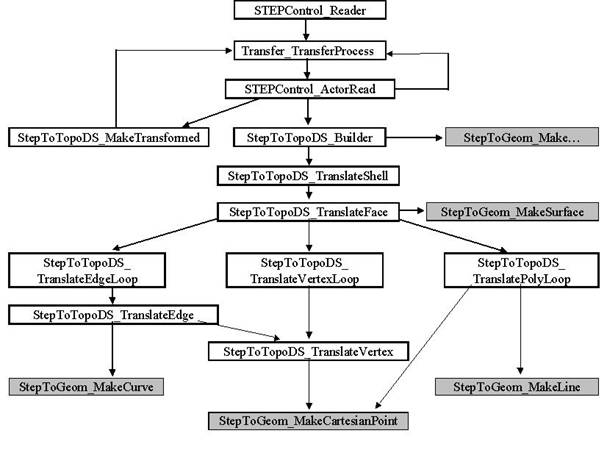
\includegraphics[width=\textwidth,height=\textheight/2,keepaspectratio=true]{step_image003.png}
\end{center}
\caption{The structure of calls in reading S\+T\+EP}
\end{DoxyImage}
 \hypertarget{occt_user_guides__step_occt_step_2_7}{}\subsection{Example}\label{occt_user_guides__step_occt_step_2_7}

\begin{DoxyCode}
1 #include <STEPControl\_Reader.hxx> 
2 #include <TopoDS\_Shape.hxx> 
3 #include <BRepTools.hxx> 
4 
5 Standard\_Integer main() 
6 \{ 
7   STEPControl\_Reader reader; 
8   reader.ReadFile(;MyFile.stp;); 
9 
10   // Loads file MyFile.stp 
11   Standard\_Integer NbRoots = reader.NbRootsForTransfer(); 
12 
13   // gets the number of transferable roots 
14   cout;Number of roots in STEP file: ; NbRootsendl; 
15 
16   Standard\_Integer NbTrans = reader.TransferRoots(); 
17   // translates all transferable roots, and returns the number of    //successful translations 
18   cout;STEP roots transferred: ; NbTransendl; 
19   cout;Number of resulting shapes is: ;reader.NbShapes()endl; 
20 
21   TopoDS\_Shape result = reader.OneShape(); 
22   // obtain the results of translation in one OCCT shape 
23 
24   . . . 
25 
26 \} 
\end{DoxyCode}
\hypertarget{occt_user_guides__step_occt_step_3}{}\section{Writing S\+T\+EP}\label{occt_user_guides__step_occt_step_3}
\hypertarget{occt_user_guides__step_occt_step_3_1}{}\subsection{Procedure}\label{occt_user_guides__step_occt_step_3_1}
You can translate O\+C\+CT shapes into S\+T\+EP entities in the following steps\+: 1.\+initialize the process, 2.\+set the translation parameters, 3.\+perform the shape translation, 4.\+write the output file.

You can translate several shapes before writing a file. All these translations output a separate shape\+\_\+representation entity in S\+T\+EP file.

The user-\/defined option (parameter {\itshape write.\+step.\+schema}) is provided to define which version of schema (A\+P214 CD or D\+IS, or A\+P203) is used for the output S\+T\+EP file.\hypertarget{occt_user_guides__step_occt_step_3_2}{}\subsection{Domain covered}\label{occt_user_guides__step_occt_step_3_2}
\hypertarget{occt_user_guides__step_occt_step_3_2_1}{}\subsubsection{Writing geometry and topology}\label{occt_user_guides__step_occt_step_3_2_1}
There are two families of O\+C\+CT objects that can be translated\+:
\begin{DoxyItemize}
\item geometrical objects,
\item topological shapes.
\end{DoxyItemize}\hypertarget{occt_user_guides__step_occt_step_3_2_2}{}\subsubsection{Writing assembly structures}\label{occt_user_guides__step_occt_step_3_2_2}
The shapes organized in a structure of nested compounds can be translated either as simple compound shapes, or into the assembly structure, depending on the parameter {\itshape write.\+step.\+assembly}, which is described below.

The assembly structure placed in the produced S\+T\+EP file corresponds to the structure described in the Pro\+S\+T\+EP Agreement Log (item 21) as the second alternative (assembly structure through {\itshape representation\+\_\+relationship} / {\itshape item\+\_\+defined\+\_\+transformation}). To represent an assembly it uses entities of the {\itshape representation\+\_\+relationship\+\_\+with\+\_\+transformation} type. Transformation operators used for locating assembly components are represented by {\itshape item\+\_\+defined\+\_\+transformation} entities. If mode {\itshape write.\+step.\+assembly} is set to the values {\itshape ON} or {\itshape Auto} then an O\+CC shape consisting of nested compounds will be written as an assembly, otherwise it will be written as separate solids.

Please see also \href{#occt_step_3_4}{\tt Mapping O\+C\+CT shapes to S\+T\+EP entities}\hypertarget{occt_user_guides__step_occt_step_3_3}{}\subsection{Description of the process}\label{occt_user_guides__step_occt_step_3_3}
\hypertarget{occt_user_guides__step_occt_step_3_3_1}{}\subsubsection{Initializing the process}\label{occt_user_guides__step_occt_step_3_3_1}
Before performing any other operation you have to create a writer object\+: 
\begin{DoxyCode}
1 STEPControl\_Writer writer; 
\end{DoxyCode}
 \hypertarget{occt_user_guides__step_occt_step_3_3_2}{}\subsubsection{Setting the translation parameters}\label{occt_user_guides__step_occt_step_3_3_2}
The following parameters are used for the O\+C\+C\+T-\/to-\/\+S\+T\+EP translation.

\subparagraph*{write.\+precision.\+mode}

writes the precision value.
\begin{DoxyItemize}
\item Least (-\/1) \+: the uncertainty value is set to the minimum tolerance of an O\+C\+CT shape
\item Average (0) \+: the uncertainty value is set to the average tolerance of an O\+C\+CT shape.
\item Greatest (1) \+: the uncertainty value is set to the maximum tolerance of an O\+C\+CT shape
\item Session (2) \+: the uncertainty value is that of the write.\+precision.\+val parameter.
\end{DoxyItemize}

Read this parameter with\+:

Standard\+\_\+\+Integer ic = Interface\+\_\+\+Static\+::\+I\+Val(\char`\"{}write.\+precision.\+mode\char`\"{}); Modify this parameter with\+: 
\begin{DoxyCode}
1 if(!Interface\_Static::SetIVal("write.precision.mode",1))  
2 .. error .. 
\end{DoxyCode}
 Default value is 0.

\subparagraph*{write.\+precision.\+val}

a user-\/defined precision value. This parameter gives the uncertainty for S\+T\+EP entities constructed from O\+C\+CT shapes when the write.\+precision.\+mode parameter value is 1.
\begin{DoxyItemize}
\item 0.\+0001\+: default
\item any real positive (non null) value.
\end{DoxyItemize}

This value is stored in shape\+\_\+representation in a S\+T\+EP file as an uncertainty.

Read this parameter with\+: 
\begin{DoxyCode}
1 Standard\_Real rp = Interface\_Static::RVal("write.precision.val");  
\end{DoxyCode}


Modify this parameter with\+: 
\begin{DoxyCode}
1 if(!Interface\_Static::SetRVal("write.precision.val",0.01))  
2 .. error .. 
\end{DoxyCode}
 Default value is 0.\+0001.

\subparagraph*{write.\+step.\+assembly}

writing assembly mode.
\begin{DoxyItemize}
\item 0 (Off) \+: (default) writes S\+T\+EP files without assemblies.
\item 1 (On) \+: writes all shapes in the form of S\+T\+EP assemblies.
\item 2 (Auto) \+: writes shapes having a structure of (possibly nested) {\itshape Topo\+D\+S\+\_\+\+Compounds} in the form of S\+T\+EP assemblies, single shapes are written without assembly structures.
\end{DoxyItemize}

Read this parameter with\+: 
\begin{DoxyCode}
1 Standard\_Integer rp = Interface\_Static::IVal("write.step.assembly"); 
\end{DoxyCode}
 Modify this parameter with\+: 
\begin{DoxyCode}
1 if(!Interface\_Static::SetIVal("write.step.assembly",1))  
2 .. error .. 
\end{DoxyCode}
 Default value is 0.

\subparagraph*{write.\+step.\+schema}

defines the version of schema used for the output S\+T\+EP file\+:
\begin{DoxyItemize}
\item 1 or ;A\+P214\+CD; (default)\+: A\+P214, CD version (dated 26 November 1996),
\item 2 or ;A\+P214\+D\+IS;\+: A\+P214, D\+IS version (dated 15 September 1998).
\item 3 or ;A\+P203;\+: A\+P203, possibly with modular extensions (depending on data written to a file).
\item 4 or {\itshape A\+P214\+IS}\+: A\+P214, IS version (dated 2002)
\end{DoxyItemize}

Read this parameter with\+: 
\begin{DoxyCode}
1 TCollection\_AsciiString schema = Interface\_Static::CVal("write.step.schema"); 
\end{DoxyCode}
 Modify this parameter with\+: 
\begin{DoxyCode}
1 if(!Interface\_Static::SetCVal("write.step.schema","DIS"))  
2 .. error .. 
\end{DoxyCode}
 Default value is 1 (;CD;). For the parameter {\itshape write.\+step.\+schema} to take effect, method {\itshape S\+T\+E\+P\+Control\+\_\+\+Writer\+::\+Model(\+Standard\+\_\+\+True)} should be called after changing this parameter (corresponding command in D\+R\+AW is {\itshape newmodel}).

\subparagraph*{write.\+step.\+product.\+name}

Defines the text string that will be used for field ‘name’ of P\+R\+O\+D\+U\+CT entities written to the S\+T\+EP file.

Default value\+: O\+C\+CT S\+T\+EP translator (current O\+C\+CT version number).

\subparagraph*{write.\+surfacecurve.\+mode}

This parameter indicates whether parametric curves (curves in parametric space of surface) should be written into the S\+T\+EP file. This parameter can be set to Off in order to minimize the size of the resulting S\+T\+EP file.


\begin{DoxyItemize}
\item Off (0) \+: writes S\+T\+EP files without pcurves. This mode decreases the size of the resulting S\+T\+EP file .
\item On (1) \+: (default) writes pcurves to S\+T\+EP file
\end{DoxyItemize}

Read this parameter with\+: 
\begin{DoxyCode}
1 Standard\_Integer wp = Interface\_Static::IVal("write.surfacecurve.mode"); 
\end{DoxyCode}
 Modify this parameter with\+: 
\begin{DoxyCode}
1 if(!Interface\_Static::SetIVal("write.surfacecurve.mode",1))  
2 .. error .. 
\end{DoxyCode}
 Default value is On.

\subparagraph*{write.\+step.\+unit}

Defines a unit in which the S\+T\+EP file should be written. If set to unit other than MM, the model is converted to these units during the translation.

Default value is MM.

\subparagraph*{write.\+step.\+resource.\+name and write.\+step.\+sequence}

These two parameters define the name of the resource file and the name of the sequence of operators (defined in that file) for Shape Processing, which is automatically performed by the S\+T\+EP translator before translating a shape to a S\+T\+EP file. Shape Processing is a user-\/configurable step, which is performed before the translation and consists in applying a set of operators to a resulting shape. This is a very powerful tool allowing customizing the shape and adapting it to the needs of a receiving application. By default the sequence consists of two operators\+: Split\+Common\+Vertex and Direct\+Faces, which convert some geometry and topological constructs valid in Open C\+A\+S\+C\+A\+DE Technology but not in S\+T\+EP to equivalent definitions conforming to S\+T\+EP format.

See description of parameter read.\+step.\+resource.\+name above for more details on using resource files.

Default values\+:
\begin{DoxyItemize}
\item read.\+step.\+resource.\+name -\/ S\+T\+EP,
\item read.\+step.\+sequence -\/ To\+S\+T\+EP.
\end{DoxyItemize}

\subparagraph*{write.\+step.\+vertex.\+mode}

This parameter indicates which of free vertices writing mode is switch on.
\begin{DoxyItemize}
\item 0 (One Compound) \+: (default) All free vertices are united into one compound and exported in one S\+H\+A\+PE D\+E\+F\+I\+N\+I\+T\+I\+ON R\+E\+P\+R\+E\+S\+E\+N\+T\+A\+T\+I\+ON (vertex name and style are lost).
\item 1 (Single Vertex) \+: Each vertex exported in its own S\+H\+A\+PE D\+E\+F\+I\+N\+I\+T\+I\+ON R\+E\+P\+R\+E\+S\+E\+N\+T\+A\+T\+I\+ON (vertex name and style are not lost, but size of S\+T\+EP file increases).
\end{DoxyItemize}

Read this parameter with\+: 
\begin{DoxyCode}
1 Standard\_Integer ic = Interface\_Static::IVal("write.step.vertex.mode"); 
\end{DoxyCode}
 Modify this parameter with\+: 
\begin{DoxyCode}
1 if(!Interface\_Static::SetIVal("write.step.vertex.mode",1))  
2 .. error .. 
\end{DoxyCode}
 Default value is 0.\hypertarget{occt_user_guides__step_occt_step_3_3_3}{}\subsubsection{Performing the Open C\+A\+S\+C\+A\+D\+E Technology shape translation}\label{occt_user_guides__step_occt_step_3_3_3}
An O\+C\+CT shape can be translated to S\+T\+EP using one of the following models (shape\+\_\+representations)\+:
\begin{DoxyItemize}
\item manifold\+\_\+solid\+\_\+brep (advanced\+\_\+brep\+\_\+shape\+\_\+representation)
\item brep\+\_\+with\+\_\+voids (advanced\+\_\+brep\+\_\+shape\+\_\+representation)
\item faceted\+\_\+brep (faceted\+\_\+brep\+\_\+shape\+\_\+representation)
\item shell\+\_\+based\+\_\+surface\+\_\+model (manifold\+\_\+surface\+\_\+shape\+\_\+representation)
\item geometric\+\_\+curve\+\_\+set (geometrically\+\_\+bounded\+\_\+wireframe\+\_\+shape\+\_\+representation)
\end{DoxyItemize}

The enumeration {\itshape S\+T\+E\+P\+Control\+\_\+\+Step\+Model\+Type} is intended to define a particular transferring model. The following values of enumeration are allowed\+:
\begin{DoxyItemize}
\item {\itshape S\+T\+E\+P\+Control\+\_\+\+As\+Is} Translator selects the resulting representation automatically, according to the type of C\+A\+S\+C\+A\+DE shape to translate it in its highest possible model;
\item {\itshape S\+T\+E\+P\+Control\+\_\+\+Manifold\+Solid\+Brep} resulting entity is manifold\+\_\+solid\+\_\+brep or brep\+\_\+with\+\_\+voids
\item {\itshape S\+T\+E\+P\+Control\+\_\+\+Faceted\+Brep} resulting entity is {\itshape faceted\+\_\+brep} or {\itshape faceted\+\_\+brep\+\_\+and\+\_\+brep\+\_\+with\+\_\+voids} Note that only planar-\/face shapes with linear edges can be written;
\item {\itshape S\+T\+E\+P\+Control\+\_\+\+Shell\+Based\+Surface\+Model} resulting entity is {\itshape shell\+\_\+based\+\_\+surface\+\_\+model};
\item {\itshape S\+T\+E\+P\+Control\+\_\+\+Geometric\+Curve\+Set} resulting entity is {\itshape geometric\+\_\+curve\+\_\+set};
\end{DoxyItemize}

The following list shows which shapes can be translated in which mode\+:
\begin{DoxyItemize}
\item {\itshape S\+T\+E\+P214\+Control\+\_\+\+As\+Is} -\/ any O\+C\+CT shape
\item {\itshape S\+T\+E\+P214\+Control\+\_\+\+Manifold\+Solid\+Brep} -\/ {\itshape Topo\+D\+S\+\_\+\+Solid, Topo\+D\+S\+\_\+\+Shell, Topo\+D\+S\+\_\+\+Compound} (if it contains {\itshape Topo\+D\+S\+\_\+\+Solids} and {\itshape Topo\+D\+S\+\_\+\+Shells}.
\item {\itshape S\+T\+E\+P214\+Control\+\_\+\+Faceted\+Brep} -\/ {\itshape Topo\+D\+S\+\_\+\+Solid} or {\itshape Topo\+D\+S\+\_\+\+Compound} containing {\itshape Topo\+D\+S\+\_\+\+Solids} if all its surfaces are {\itshape Geom\+\_\+\+Planes} and all curves are {\itshape Geom\+\_\+\+Lines}.
\item {\itshape S\+T\+E\+P214\+Control\+\_\+\+Shell\+Based\+Surface\+Model} -\/ {\itshape Topo\+D\+S\+\_\+\+Solid, Topo\+D\+S\+\_\+\+Shell, Topo\+D\+S\+\_\+\+Face} and {\itshape Topo\+D\+S\+\_\+\+Compound} (if it contains all mentioned shapes)
\item {\itshape S\+T\+E\+P214\+Control\+\_\+\+Geometric\+Curve\+Set} -\/ any O\+C\+CT shape.
\end{DoxyItemize}

If {\itshape Topo\+D\+S\+\_\+\+Compound} contains any other types besides the ones mentioned in the table, these sub-\/shapes will be ignored.

In case if an O\+C\+CT shape cannot be translated according to its mode the result of translation is void. 
\begin{DoxyCode}
1 STEP214Control\_StepModelTope mode = STEP214Control\_ManifoldSolidBrep; 
2 IFSelect\_ReturnStatus stat = writer.Transfer(shape,mode); 
\end{DoxyCode}
\hypertarget{occt_user_guides__step_occt_step_3_3_4}{}\subsubsection{Writing the S\+T\+E\+P file}\label{occt_user_guides__step_occt_step_3_3_4}
Write the S\+T\+EP file with\+: 
\begin{DoxyCode}
1 IFSelect\_ReturnStatus stat = writer.Write("filename.stp"); 
\end{DoxyCode}
 to give the file name.\hypertarget{occt_user_guides__step_occt_step_3_4}{}\subsection{Mapping Open C\+A\+S\+C\+A\+D\+E Technology shapes to S\+T\+E\+P entities}\label{occt_user_guides__step_occt_step_3_4}
Only S\+T\+EP entities that have a corresponding O\+C\+CT object and mapping of assembly structures are described in this paragraph. For a full list of S\+T\+EP entities please refer to Appendix A.\hypertarget{occt_user_guides__step_occt_step_3_4_1}{}\subsubsection{Assembly structures and product information}\label{occt_user_guides__step_occt_step_3_4_1}
The assembly structures are written to the S\+T\+EP file if parameter {\itshape write.\+step.\+assembly} is 1 or 2. Each {\itshape Topo\+D\+S\+\_\+\+Compound} is written as an assembly with subshapes of that compound being components of the assembly. The structure of nested compounds is translated to the structure of nested assemblies. Shared subshapes are translated into shared components of assemblies. Shapes that are not compounds are translated into subtypes of shape\+\_\+representation according to their type (see the next subchapter for details).

A set of S\+T\+EP entities describing general product information is written to the S\+T\+EP file together with the entities describing the product geometry, topology and assembly structure. Most of these entities are attached to the entities being subtypes of shape\+\_\+representation, but some of them are created only one per S\+T\+EP file.

The table below describes S\+T\+EP entities, which are created when the assembly structure and product information are written to the S\+T\+EP file, and shows how many of these entities are created. Note that the appearance of some of these entities depends on the version of the schema (A\+P214, CD, D\+IS or IS, or A\+P203).

\tabulinesep=1mm
\begin{longtabu} spread 0pt [c]{*3{|X[-1]}|}
\hline
\rowcolor{\tableheadbgcolor}{\bf C\+A\+S\+C\+A\+DE shape }&{\bf S\+T\+EP entity }&{\bf Comments  }\\\cline{1-3}
\endfirsthead
\hline
\endfoot
\hline
\rowcolor{\tableheadbgcolor}{\bf C\+A\+S\+C\+A\+DE shape }&{\bf S\+T\+EP entity }&{\bf Comments  }\\\cline{1-3}
\endhead
&application\+\_\+protocol\+\_\+definition &One per S\+T\+EP file, defines the application protocol used (depends on the schema version) \\\cline{1-3}
&application\+\_\+context &One per S\+T\+EP file, defines the application generating the file (A\+P214 or A\+P203) \\\cline{1-3}
Topo\+D\+S\+\_\+\+Compound &shape\+\_\+representation &Empty {\itshape shape\+\_\+representation} describing the assembly. The components of that assembly are written as subtypes of shape\+\_\+representation and are included to the assembly using {\itshape next\+\_\+assembly\+\_\+usage\+\_\+occurence} entities. \\\cline{1-3}
Topo\+D\+S\+\_\+\+Shape &subtypes of shape\+\_\+representation &Depending on the shape type, see the tables below for mapping details \\\cline{1-3}
&next\+\_\+assembly\+\_\+usage\+\_\+occurence &Describes the instance of component in the assembly by referring corresponding {\itshape product\+\_\+definitions}. If the same component is included in the assembly several times (for example, with different locations), several {\itshape next\+\_\+assembly\+\_\+usage\+\_\+occurences} are created. \\\cline{1-3}
&context\+\_\+dependent\+\_\+shape\+\_\+representation &Describes the placement of a component in the assembly. One {\itshape context\+\_\+dependent\+\_\+shape\+\_\+representation} corresponds to each {\itshape next\+\_\+assembly\+\_\+usage\+\_\+occurence} entity. \\\cline{1-3}
&shape\+\_\+representation\+\_\+relationship\+\_\+with\+\_\+transformation &Together with the {\itshape context\+\_\+dependent\+\_\+shape\+\_\+representation} describes the location of a component in the assembly. \\\cline{1-3}
&item\+\_\+defined\+\_\+transformation &Defines a transformation used for the location of a component in the assembly. Is referred by {\itshape shape\+\_\+representation\+\_\+relationship\+\_\+with\+\_\+transformation}. \\\cline{1-3}
&shape\+\_\+definition\+\_\+representation &One per {\itshape shape\+\_\+representation}. \\\cline{1-3}
&product\+\_\+definition\+\_\+shape &One per {\itshape shape\+\_\+definition\+\_\+representation} and {\itshape context\+\_\+dependent\+\_\+shape\+\_\+representation} \\\cline{1-3}
&product\+\_\+definition &Defines a product, one per {\itshape shape\+\_\+definition\+\_\+representation} \\\cline{1-3}
&product\+\_\+definition\+\_\+formation &One per {\itshape product\+\_\+definition}. All {\itshape product\+\_\+definition\+\_\+formations} in the S\+T\+EP file have unique names. \\\cline{1-3}
&Product &One per {\itshape product\+\_\+definition\+\_\+formation}. All products in the S\+T\+EP file have unique names. \\\cline{1-3}
&product\+\_\+type (CD) or product\+\_\+related\+\_\+product\+\_\+category (D\+IS,IS) &One per product \\\cline{1-3}
&Mechanical\+\_\+context (CD) or product\+\_\+context (D\+IS,IS) &One per product. \\\cline{1-3}
&product\+\_\+definition\+\_\+context &One per {\itshape product\+\_\+definition}. \\\cline{1-3}
\end{longtabu}
\hypertarget{occt_user_guides__step_occt_step_3_4_2}{}\subsubsection{Topological shapes}\label{occt_user_guides__step_occt_step_3_4_2}
\tabulinesep=1mm
\begin{longtabu} spread 0pt [c]{*3{|X[-1]}|}
\hline
\rowcolor{\tableheadbgcolor}{\bf C\+A\+S\+C\+A\+DE shape }&{\bf S\+T\+EP entity }&{\bf Comments  }\\\cline{1-3}
\endfirsthead
\hline
\endfoot
\hline
\rowcolor{\tableheadbgcolor}{\bf C\+A\+S\+C\+A\+DE shape }&{\bf S\+T\+EP entity }&{\bf Comments  }\\\cline{1-3}
\endhead
Topo\+D\+S\+\_\+\+Compound &geometric\+\_\+curve\+\_\+set &If the write mode is {\itshape S\+T\+E\+P214\+Control\+\_\+\+Geometric\+Curve\+Set} only 3D curves of the edges found in {\itshape Topo\+D\+S\+\_\+\+Compound} and all its subshapes are translated \\\cline{1-3}
&manifold\+\_\+solid\+\_\+brep &If the write mode is {\itshape S\+T\+E\+P214\+Control\+\_\+\+As\+Is} and {\itshape Topo\+D\+S\+\_\+\+Compound} consists only of {\itshape Topo\+D\+S\+\_\+\+Solids}. \\\cline{1-3}
&shell\+\_\+based\+\_\+surface\+\_\+model &If the write mode is {\itshape S\+T\+E\+P214\+Control\+\_\+\+As\+Is} and {\itshape Topo\+D\+S\+\_\+\+Compound} consists of {\itshape Topo\+D\+S\+\_\+\+Solids}, {\itshape Topo\+D\+S\+\_\+\+Shells} and {\itshape Topo\+D\+S\+\_\+\+Faces}. \\\cline{1-3}
&geometric\+\_\+curve\+\_\+set &If the write mode is {\itshape S\+T\+E\+P214\+Control\+\_\+\+As\+Is} and {\itshape Topo\+D\+S\+\_\+\+Compound} contains {\itshape Topo\+D\+S\+\_\+\+Wires, Topo\+D\+S\+\_\+\+Edges, Topo\+D\+S\+\_\+\+Vertices}. If the write mode is not {\itshape S\+T\+E\+P214\+Control\+\_\+\+As\+Is} or {\itshape S\+T\+E\+P214\+Control\+\_\+\+Geometric\+Curve\+Set}, {\itshape Topo\+D\+S\+\_\+\+Solids, Topo\+D\+S\+\_\+\+Shells} and {\itshape Topo\+D\+S\+\_\+\+Faces} are translated according to this table. \\\cline{1-3}
Topo\+D\+S\+\_\+\+Solid &manifold\+\_\+solid\+\_\+brep &If the write mode is {\itshape S\+T\+E\+P214\+Control\+\_\+\+As\+Is} or {\itshape S\+T\+E\+P214\+Control\+\_\+\+Manifold\+Solid\+Brep} and C\+A\+S\+C\+A\+DE {\itshape Topo\+D\+S\+\_\+\+Solid} has no voids. \\\cline{1-3}
&faceted\+\_\+brep &If the write mode is {\itshape S\+T\+E\+P214\+Control\+\_\+\+Faceted\+Brep}. \\\cline{1-3}
&brep\+\_\+with\+\_\+voids &If the write mode is {\itshape S\+T\+E\+P214\+Control\+\_\+\+As\+Is} or {\itshape S\+T\+E\+P214\+Control\+\_\+\+Manifold\+Solid\+Brep} and C\+A\+S\+C\+A\+DE {\itshape Topo\+D\+S\+\_\+\+Solid} has voids. \\\cline{1-3}
&shell\+\_\+based\+\_\+surface\+\_\+model &If the write mode is {\itshape S\+T\+E\+P214\+Control\+\_\+\+Shell\+Based\+Surface\+Model}. \\\cline{1-3}
&geometric\+\_\+curve\+\_\+set &If the write mode is {\itshape S\+T\+E\+P214\+Control\+\_\+\+Geometric\+Curve\+Set}. Only 3D curves of the edges are translated. \\\cline{1-3}
Topo\+D\+S\+\_\+\+Shell in a Topo\+D\+S\+\_\+\+Solid &closed\+\_\+shell &If {\itshape Topo\+D\+S\+\_\+\+Shell} is closed shell. \\\cline{1-3}
Topo\+D\+S\+\_\+\+Shell &manifold\+\_\+solid\+\_\+brep &If the write mode is {\itshape S\+T\+E\+P214\+Control\+\_\+\+Manifold\+Solid\+Brep}. \\\cline{1-3}
&shell\+\_\+based\+\_\+surface\+\_\+model &If the write mode is {\itshape S\+T\+E\+P214\+Control\+\_\+\+As\+Is} or {\itshape S\+T\+E\+P214\+Control\+\_\+\+Shell\+Based\+Surface\+Model}. \\\cline{1-3}
&geometric\+\_\+curve\+\_\+set &If the write mode is {\itshape S\+T\+E\+P214\+Control\+\_\+\+Geometric\+Curve\+Set}. Only 3D curves of the edges are translated. \\\cline{1-3}
Topo\+D\+S\+\_\+\+Face &advanced\+\_\+face &\\\cline{1-3}
Topo\+D\+S\+\_\+\+Wire in a Topo\+D\+S\+\_\+\+Face &face\+\_\+bound &The resulting {\itshape face\+\_\+bound} contains {\itshape poly\+\_\+loop} if write mode is {\itshape faceted\+\_\+brep} or {\itshape edge\+\_\+loop} if it is not. \\\cline{1-3}
Topo\+D\+S\+\_\+\+Wire &geometric\+\_\+curve\+\_\+set &If the write mode is {\itshape S\+T\+E\+P214\+Control\+\_\+\+Geometric\+Curve\+Set}. Only 3D curves of the edges are translated. \\\cline{1-3}
Topo\+D\+S\+\_\+\+Edge &oriented\+\_\+edge &\\\cline{1-3}
Topo\+D\+S\+\_\+\+Vertex &vertex\+\_\+point &\\\cline{1-3}
\end{longtabu}
\hypertarget{occt_user_guides__step_occt_step_3_4_3}{}\subsubsection{Geometrical objects}\label{occt_user_guides__step_occt_step_3_4_3}
\tabulinesep=1mm
\begin{longtabu} spread 0pt [c]{*4{|X[-1]}|}
\hline
\rowcolor{\tableheadbgcolor}{\bf Geometry }&{\bf C\+A\+S\+C\+A\+DE object }&{\bf S\+T\+EP entity }&{\bf Comments  }\\\cline{1-4}
\endfirsthead
\hline
\endfoot
\hline
\rowcolor{\tableheadbgcolor}{\bf Geometry }&{\bf C\+A\+S\+C\+A\+DE object }&{\bf S\+T\+EP entity }&{\bf Comments  }\\\cline{1-4}
\endhead
Points &Geom\+\_\+\+Cartesian\+Point, Geom2d\+\_\+\+Cartesian\+Point &cartesian\+\_\+point &\\\cline{1-4}
&T\+Colgp\+\_\+\+Array1\+Of\+Pnt, T\+Colgp\+\_\+\+Array1\+Of\+Pnt2d &polyline &\\\cline{1-4}
Placements &Geom\+\_\+\+Axis1\+Plasement, Geom2d\+\_\+\+Axis\+Placement &axis1\+\_\+placement &\\\cline{1-4}
&Geom\+\_\+\+Axis2\+Placement &axis2\+\_\+placement\+\_\+3d &\\\cline{1-4}
Directions &Geom\+\_\+\+Direction, Geom2d\+\_\+\+Direction &direction &\\\cline{1-4}
Vectors &Geom\+\_\+\+Vector, Geom2d\+\_\+\+Vector &vector &\\\cline{1-4}
Curves &Geom\+\_\+\+Circle &circle &\\\cline{1-4}
&Geom2d\+\_\+\+Circle &circle, rational\+\_\+b\+\_\+spline\+\_\+curve &\\\cline{1-4}
&Geom\+\_\+\+Ellipse &Ellipse &\\\cline{1-4}
&Geom2d\+\_\+\+Ellipse &Ellipse, rational\+\_\+b\+\_\+spline\+\_\+curve &\\\cline{1-4}
&Geom\+\_\+\+Hyperbola, Geom2d\+\_\+\+Hyperbola &Hyperbola &\\\cline{1-4}
&Geom\+\_\+\+Parabola, Geom2d\+\_\+\+Parabola &Parabola &\\\cline{1-4}
&Geom\+\_\+\+B\+Spline\+Curve &b\+\_\+spline\+\_\+curve\+\_\+with\+\_\+knots or rational\+\_\+b\+\_\+spline\+\_\+curve &{\itshape rational\+\_\+b\+\_\+spline\+\_\+curve} is produced if {\itshape Geom\+\_\+\+Bspline\+Curve} is a rational B\+Spline \\\cline{1-4}
&Geom2d\+\_\+\+B\+Spline\+Curve &b\+\_\+spline\+\_\+curve\+\_\+with\+\_\+knots or rational\+\_\+b\+\_\+spline\+\_\+curve &{\itshape rational\+\_\+b\+\_\+spline\+\_\+curve} is produced if {\itshape Geom2d\+\_\+\+Bspline\+Curve} is a rational B\+Spline \\\cline{1-4}
&Geom\+\_\+\+Bezier\+Curve &b\+\_\+spline\+\_\+curve\+\_\+with\+\_\+knots &\\\cline{1-4}
&Geom\+\_\+\+Line or Geom2d\+\_\+\+Line &Line &\\\cline{1-4}
Surfaces &Geom\+\_\+\+Plane &Plane &\\\cline{1-4}
&Geom\+\_\+\+Offset\+Surface &offset\+\_\+surface &\\\cline{1-4}
&Geom\+\_\+\+Conical\+Surface &conical\+\_\+surface &\\\cline{1-4}
&Geom\+\_\+\+Cylindrical\+Surface &cylindrical\+\_\+surface &\\\cline{1-4}
&Geom\+\_\+\+Offset\+Surface &offset\+\_\+surface &\\\cline{1-4}
&Geom\+\_\+\+Rectangular\+Trimmed\+Surface &rectangular\+\_\+trimmed\+\_\+surface &\\\cline{1-4}
&Geom\+\_\+\+Spherical\+Surface &spherical\+\_\+surface &\\\cline{1-4}
&Geom\+\_\+\+Surface\+Of\+Linear Extrusion &surface\+\_\+of\+\_\+linear\+\_\+extrusion &\\\cline{1-4}
&Geom\+\_\+\+Surface\+Of Revolution &surface\+\_\+of\+\_\+revolution &\\\cline{1-4}
&Geom\+\_\+\+Toroidal\+Surface &toroidal\+\_\+surface or degenerate\+\_\+toroidal\+\_\+surface &{\itshape degenerate\+\_\+toroidal\+\_\+surface} is produced if the minor radius is greater then the major one \\\cline{1-4}
&Geom\+\_\+\+Bezier\+Surface &b\+\_\+spline\+\_\+surface\+\_\+with\+\_\+knots &\\\cline{1-4}
&Geom\+\_\+\+Bspline\+Surface &b\+\_\+spline\+\_\+surface\+\_\+with\+\_\+knots or rational\+\_\+b\+\_\+spline\+\_\+surface &{\itshape rational\+\_\+b\+\_\+spline\+\_\+surface} is produced if {\itshape Geom\+\_\+\+B\+Spline\+Surface} is a rational Bspline \\\cline{1-4}
\end{longtabu}
\hypertarget{occt_user_guides__step_occt_step_3_5}{}\subsection{Tolerance management}\label{occt_user_guides__step_occt_step_3_5}
There are four possible values for the uncertainty when writing a S\+T\+EP file\+:
\begin{DoxyItemize}
\item user-\/defined value of the uncertainty
\item minimal value of sub-\/shapes tolerances
\item average value of sub-\/shapes tolerances
\item maximal value of sub-\/shapes tolerances
\end{DoxyItemize}

The chosen value of the uncertainty is the final value that will be written into the S\+T\+EP file. See parameter {\itshape write.\+precision.\+mode}.\hypertarget{occt_user_guides__step_occt_step_3_6}{}\subsection{Code architecture}\label{occt_user_guides__step_occt_step_3_6}
\hypertarget{occt_user_guides__step_occt_step_3_6_1}{}\subsubsection{Graph of calls}\label{occt_user_guides__step_occt_step_3_6_1}
The following diagram illustrates the structure of calls in writing S\+T\+EP. The highlighted classes are intended to translate geometry.


\begin{DoxyImage}
\begin{center}
 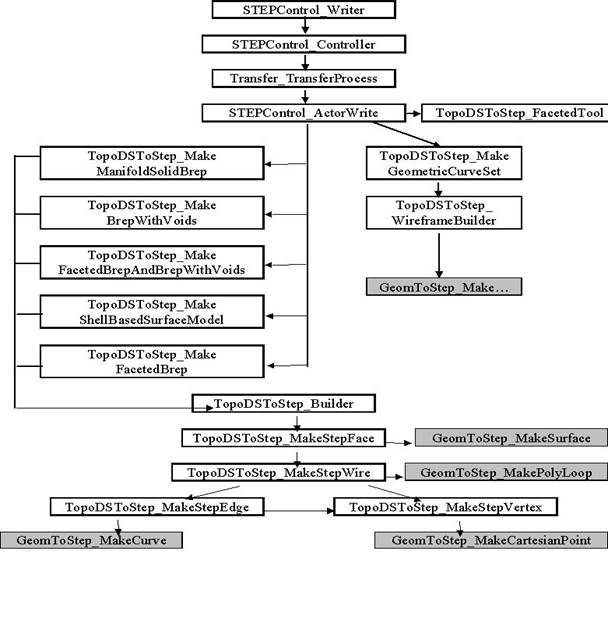
\includegraphics[width=\textwidth,height=\textheight/2,keepaspectratio=true]{step_image004.png}
\end{center}
\caption{The structure of calls in writing S\+T\+EP}
\end{DoxyImage}
\hypertarget{occt_user_guides__step_occt_step_3_7}{}\subsection{Example}\label{occt_user_guides__step_occt_step_3_7}

\begin{DoxyCode}
\textcolor{preprocessor}{#include <STEPControl.hxx>} 
\textcolor{preprocessor}{#include <STEPControl\_Writer.hxx>} 
\textcolor{preprocessor}{#include <TopoDS\_Shape.hxx>} 
\textcolor{preprocessor}{#include <BRepTools.hxx>} 
\textcolor{preprocessor}{#include <BRep\_Builder.hxx>} 

Standard\_Integer main() 
\{ 
TopoDS\_Solid source; 
. . . 

STEPControl\_Writer writer; 
writer.Transfer(source, STEPControl\_ManifoldSolidBrep); 

\textcolor{comment}{// Translates TopoDS\_Shape into manifold\_solid\_brep entity }
writer.Write(;Output.stp;); 
\textcolor{comment}{// writes the resulting entity in the STEP file }

\} 
\end{DoxyCode}
\hypertarget{occt_user_guides__step_occt_step_4}{}\section{Physical S\+T\+E\+P file reading and writing}\label{occt_user_guides__step_occt_step_4}
\hypertarget{occt_user_guides__step_occt_step_4_1}{}\subsection{Architecture of S\+T\+E\+P Read and Write classes}\label{occt_user_guides__step_occt_step_4_1}
\hypertarget{occt_user_guides__step_occt_step_4_1_1}{}\subsubsection{General principles}\label{occt_user_guides__step_occt_step_4_1_1}
To perform data loading from a S\+T\+EP file and to translate this data it is necessary to create correspondence between the E\+X\+P\+R\+E\+SS schema and the structure of C\+DL classes. There are two possibilities to organize such correspondence\+: the so-\/called early binding and late binding.
\begin{DoxyItemize}
\item Late binding means that the processor works with a description of the schema. The processor builds a dictionary of entities and can recognize and read any entity that is described in the schema. To change the behavior and the scope of processor based on late binding it is enough to change the description of the schema. However, this binding has some disadvantages (for example low speed of reading process).
\item In case of early binding, the structure of C\+DL classes is created beforehand with the help of a specific automatic tool or manually. If the processor finds an entity that is not found in this schema, it will simply be ignored. The processor calls constructors of appropriate classes and their read methods. To add a new type in the scope of the processor it is necessary to create a class corresponding to the new entity.
\end{DoxyItemize}

The S\+T\+EP processor is based on early binding principles. It means that specific classes for each E\+X\+P\+R\+E\+SS type have been created with the help of an automatic tool from the E\+X\+P\+R\+E\+SS schema. There are two C\+DL classes for each E\+X\+P\+R\+E\+SS type. The first class (named the representing class) represents the S\+T\+EP entity in memory. The second one (RW -\/ class) is intended to perform the initialization of the representing class and to output data to an intermediate structure to be written in a S\+T\+EP file.\hypertarget{occt_user_guides__step_occt_step_4_1_2}{}\subsubsection{Complex entities}\label{occt_user_guides__step_occt_step_4_1_2}
E\+X\+P\+R\+E\+SS schema allows multiple inheritance. Entities that are built on the basis of multiple inheritance are called complex entities. Multiple inheritance is not available in C\+DL. E\+X\+P\+R\+E\+SS enables any type of complex entities that can be inherited from any E\+X\+P\+R\+E\+SS type. In the manner of early binding it is not possible to create a C\+DL class for any possible complex type. Thus, only widespread complex entities have corresponding representing classes and R\+W-\/classes that are created manually beforehand.\hypertarget{occt_user_guides__step_occt_step_4_2}{}\subsection{Physical file reading}\label{occt_user_guides__step_occt_step_4_2}
Physical file reading consists of the following steps\+: 1.\+Loading a S\+T\+EP file and syntactic analysis of its contents 2.\+Mapping S\+T\+EP entities to the array of strings 3.\+Creating empty O\+C\+CT objects representing S\+T\+EP entities 4.\+Initializing O\+C\+CT objects 5.\+Building a references graph\hypertarget{occt_user_guides__step_occt_step_4_2_1}{}\subsubsection{Loading a S\+T\+E\+P file and syntactic analysis of its contents}\label{occt_user_guides__step_occt_step_4_2_1}
In the first phase, a S\+T\+EP file is syntactically checked and loaded in memory as a sequence of strings.

Syntactic check is performed on the basis of rules defined in {\itshape step.\+lex} and {\itshape step.\+yacc} files. Files {\itshape step.\+lex} and {\itshape step.\+yacc} are located in the Step\+File nocdlpack development unit. These files describe text encoding of S\+T\+EP data structure (for additional information see I\+SO 10303 Part 21). The {\itshape step.\+lex} file describes the lexical structure of the S\+T\+EP file. It describes identifiers, numbers, delimiters, etc. The {\itshape step.\+yacc} file describes the syntactic structure of the file, such as entities, parameters, and headers.

These files have been created only once and need to be updated only when norm I\+SO 10303-\/21 is changed.\hypertarget{occt_user_guides__step_occt_step_4_2_2}{}\subsubsection{Mapping S\+T\+E\+P entities to arrays of strings}\label{occt_user_guides__step_occt_step_4_2_2}
For each entity specified by its rank number the arrays storing its identifier, S\+T\+EP type and parameters are filled. \hypertarget{occt_user_guides__step_occt_step_4_2_3}{}\subsubsection{Creating empty Open C\+A\+S\+C\+A\+D\+E Technology objects that represent S\+T\+E\+P entities}\label{occt_user_guides__step_occt_step_4_2_3}
For each S\+T\+EP entity an empty O\+C\+CT object representing this entity is created. A map of correspondence between entity rank and O\+C\+CT object is created and filled out. If a S\+T\+EP entity is not recognized by the S\+T\+EP processor then the {\itshape Step\+Data\+\_\+\+Undefined\+Entity} object is created. \hypertarget{occt_user_guides__step_occt_step_4_2_4}{}\subsubsection{Initializing Open C\+A\+S\+C\+A\+D\+E Technology objects}\label{occt_user_guides__step_occt_step_4_2_4}
Each O\+C\+CT object (including Step\+Data\+\_\+\+Undefined\+Entity) is initialized by its parameters with the help of the appropriate RW -\/ class. If some entity has another entity as its parameter, the object that represents the latter entity will be initialized immediately. All initialized objects are put into a special map to avoid repeated initialization. \hypertarget{occt_user_guides__step_occt_step_4_2_5}{}\subsubsection{Building a graph}\label{occt_user_guides__step_occt_step_4_2_5}
The final phase is building a graph of references between entities. For each entity its R\+W-\/class is used to find entities referenced by this entity. Back references are built on the basis of direct references. In addition to explicit references defined in the S\+T\+EP entities some additional (implicit) references are created for entities representing assembly structures (links from assemblies to their components). \hypertarget{occt_user_guides__step_occt_step_4_3}{}\subsection{How to add a new entity in scope of the S\+T\+E\+P processor}\label{occt_user_guides__step_occt_step_4_3}
If it is necessary to read and translate a new entity by the S\+T\+EP processor the Reader and Actor scope should be enhanced. Note that some actions to be made for adding a new type are different for simple and complex types. The following steps should be taken\+:
\begin{DoxyItemize}
\item Create a C\+DL class representing a new entity. This can be {\itshape Stepxxx\+\_\+\+New\+Entity} class where xxx can be one of the following\+:
\begin{DoxyItemize}
\item Basic
\item Geom
\item Shape
\item Visual
\item Repr
\item A\+P214
\item A\+P203 Each field of a S\+T\+EP entity should be represented by a corresponding field of this class. The class should have methods for initializing, setting and obtaining fields and it should also have the default constructor.
\end{DoxyItemize}
\item Create the {\itshape R\+W\+Stepxxx\+\_\+\+R\+W\+New\+Entity} class with a default constructor and methods {\itshape Read\+Step()}, {\itshape Write\+Step()} and if the entity references other entities, then method {\itshape Share()}.
\item Update file {\itshape Step\+A\+P214\+\_\+\+Protocol.\+cxx}. In the constructor {\itshape Step\+A\+P214\+\_\+\+Protocol\+::\+Step\+A\+P214\+\_\+\+Protocol()} add the new type to the map of registered types and associate the unique integer identifier with this type.
\item Update file {\itshape R\+W\+Step\+A\+P214\+\_\+\+Read\+Write\+Module.\+cxx}. The changes should be the following\+:
\begin{DoxyItemize}
\item For simple types\+:
\begin{DoxyItemize}
\item Add a static object of class {\itshape T\+Collection\+\_\+\+Ascii\+String} with name {\itshape Reco\+\_\+\+New\+Entity} and initialize it with a string containing the S\+T\+EP type.
\item In constructor {\itshape W\+Step\+A\+P214\+\_\+\+Read\+Write\+Module\+::\+R\+W\+Step\+A\+P214\+\_\+\+Read\+Write\+Module()} add this object onto the list with the unique integer identifier of the new entity type.
\item In function {\itshape R\+W\+Step\+A\+P214\+\_\+\+Read\+Write\+Module\+::\+Step\+Type()} add a new C++ case operator for this identifier.
\end{DoxyItemize}
\item For complex types\+:
\begin{DoxyItemize}
\item In the method {\itshape R\+W\+Step\+A\+P214\+\_\+\+Read\+Write\+Module\+::\+Case\+Step()} add a code for recognition the new entity type returning its unique integer identifier.
\item In the method {\itshape R\+W\+Step\+A\+P214\+\_\+\+Read\+Write\+Module\+::\+Is\+Complex()} return True for this type.
\item In the method {\itshape R\+W\+Step\+A\+P214\+\_\+\+Read\+Write\+Module\+::\+Complex\+Type()} fill the list of subtypes composing this complex type.
\end{DoxyItemize}
\item For both simple and complex types\+:
\begin{DoxyItemize}
\item In function {\itshape R\+W\+Step\+A\+P214\+\_\+\+Read\+Write\+Module\+::\+Read\+Step()} add a new C++ case operator for the new identifier and call the {\itshape R\+W\+Stepxxx\+\_\+\+R\+W\+New\+Entity} class, method {\itshape Read\+Step} to initialize the new class.
\end{DoxyItemize}
\end{DoxyItemize}
\item Update file {\itshape R\+W\+Step\+A\+P214\+\_\+\+General\+Module.\+cxx}. Add new C++ case operators to functions {\itshape New\+Void()} and {\itshape Fill\+Shared\+Case()}, and in the method {\itshape Category\+Number()} add a line defining a category of the new type.
\item Enhance the {\itshape S\+T\+E\+P\+Control\+\_\+\+Actor\+Read class} (methods {\itshape Recognize()} and {\itshape Transfer()}), or class(es) translating some entities, to translate the new entity into an O\+C\+CT shape.
\end{DoxyItemize}\hypertarget{occt_user_guides__step_occt_step_4_4}{}\subsection{Physical file writing}\label{occt_user_guides__step_occt_step_4_4}
Physical file writing consists of the following steps\+:
\begin{DoxyEnumerate}
\item Building a references graph. Physical writing starts when S\+T\+EP model, which was either loaded from a S\+T\+EP file or created from O\+C\+CT shape with the help of translator, is available together with corresponding graph of references. During this step the graph of references can be recomputed.
\item Transferring data from a model to a sequence of strings. For each representing entity from the model a corresponding RW -\/ class is called. RW -\/ class performs the writing of data that is contained in the representing class into an intermediate data structure. The mentioned structure is a sequence of strings in memory.
\item Writing the sequence of strings into the file. The sequence of strings is written into the file. This is the last phase of physical S\+T\+EP writing.
\end{DoxyEnumerate}\hypertarget{occt_user_guides__step_occt_step_4_5}{}\subsection{How to add a new entity to write in the S\+T\+E\+P file.}\label{occt_user_guides__step_occt_step_4_5}
If it is necessary to write and translate an O\+C\+CT shape into a new entity by the S\+T\+EP processor the Writer and Actor scope should be enhanced.

For a description of steps, which should be taken for adding a new entity type to the S\+T\+EP processor, see \href{#occt_step_4_2}{\tt Physical file reading}. Then, enhance the {\itshape S\+T\+E\+P\+Control\+\_\+\+Actor\+Write} class i.\+e. methods {\itshape Recognize()} and {\itshape Transfer()}, or other classes from {\itshape Topo\+D\+S\+To\+Step}, to translate the O\+C\+CT shape into a new S\+T\+EP entity.\hypertarget{occt_user_guides__step_occt_step_6}{}\section{Using D\+R\+AW}\label{occt_user_guides__step_occt_step_6}
\hypertarget{occt_user_guides__step_occt_step_6_1}{}\subsection{D\+R\+A\+W S\+T\+E\+P Commands Overview}\label{occt_user_guides__step_occt_step_6_1}
{\itshape T\+K\+X\+S\+D\+R\+AW} toolkit provides commands for testing X\+S\+T\+EP interfaces interactively in the D\+R\+AW environment. It provides an additional set of D\+R\+AW commands specific for data exchange tasks, which allows loading and writing data files and an analysis of the resulting data structures and shapes.

This section is divided into five parts. Two of them deal with reading and writing a S\+T\+EP file and are specific for the S\+T\+EP processor. The first and the forth parts describe some general tools for setting parameters and analyzing the data. Most of them are independent of the norm being tested. Additionally, a table of mentioned D\+R\+AW commands is provided.

In the description of commands, square brackets (\mbox{[}\mbox{]}) are used to indicate optional parameters. Parameters given in the angle brackets ($<$$>$) and sharps (\#) are to be substituted by an appropriate value. When several exclusive variants are possible, a vertical dash ($\vert$) is used.\hypertarget{occt_user_guides__step_occt_step_6_2}{}\subsection{Setting the interface parameters}\label{occt_user_guides__step_occt_step_6_2}
A set of parameters for importing and exporting S\+T\+EP data is defined in the X\+S\+T\+EP resource file. In X\+S\+D\+R\+AW, these parameters can be viewed or changed using the command 
\begin{DoxyCode}
1 Draw:> param [<parameter\_name> [<value>]] 
\end{DoxyCode}
 Command {\itshape param} with no arguments gives a list of all parameters with their values. When the argument {\itshape parameter\+\_\+name} is specified, information about this parameter is printed (current value and short description).

The third argument is used to set a new value of the given parameter. The result of the setting is printed immediately.

During all interface operations, the protocol of the process (fail and warning messages, mapping of loaded entities into O\+C\+CT shapes etc.) can be output to the trace file. Two parameters are defined in the D\+R\+AW session\+: trace level (integer value from 0 to 9, default is 0), and trace file (default is standard output).

Command xtrace is intended to view and change these parameters\+:
\begin{DoxyItemize}
\item {\itshape Draw\+:$>$ xtrace} -\/ prints current settings (e.\+g.\+: `\+Level=1 -\/ Standard Output\textquotesingle{});
\item {\itshape Draw\+:$>$ xtrace \#} -\/ sets trace level to the value \#;
\item {\itshape Draw\+:$>$ xtrace tracefile.\+log} -\/ sets the trace file as {\itshape tracefile.\+log};
\item {\itshape Draw\+:$>$ xtrace.} -\/ directs all messages to the standard output.
\end{DoxyItemize}\hypertarget{occt_user_guides__step_occt_step_6_3}{}\subsection{Reading a S\+T\+E\+P file}\label{occt_user_guides__step_occt_step_6_3}
For a description of parameters used in reading a S\+T\+EP file refer to \href{#occt_step_2_3_3}{\tt Setting the translation parameters} section.

For reading a S\+T\+EP file, the following parameters are defined (see above, \href{#occt_step_6_2}{\tt the command {\itshape param}})\+:

\tabulinesep=1mm
\begin{longtabu} spread 0pt [c]{*4{|X[-1]}|}
\hline
\rowcolor{\tableheadbgcolor}{\bf Description }&{\bf Name }&{\bf Values }&{\bf Meaning  }\\\cline{1-4}
\endfirsthead
\hline
\endfoot
\hline
\rowcolor{\tableheadbgcolor}{\bf Description }&{\bf Name }&{\bf Values }&{\bf Meaning  }\\\cline{1-4}
\endhead
Precision for input entities &read.\+precision.\+mode &0 or 1 &If 0 (File), precision of the input S\+T\+EP file will be used for the loaded shapes; If 1 (Session), the following parameter will be used as the precision value. \\\cline{1-4}
&read.\+precision.\+val &real &Value of precision (used if the previous parameter is 1) \\\cline{1-4}
Surface curves &read.\+surfacecurve.\+mode &0 or 3 &Defines a preferable way of representing surface curves (2d or 3d representation). If 0, no preference. \\\cline{1-4}
Maximal tolerance &read.\+maxprecision.\+mode &0 or 1 &If 1, maximum tolerance is used as a rigid limit If 0, maximum tolerance is used as a limit but can be exceeded by some algorithms. \\\cline{1-4}
&read.\+maxprecision.\+val &real &Value of maximum precision \\\cline{1-4}
\end{longtabu}
It is possible either only to load a S\+T\+EP file into memory (i.\+e. fill the {\itshape Interface\+Model} with data from the file), or to read it (i.\+e. load and convert all entities to O\+C\+CT shapes). Loading is done by the command 
\begin{DoxyCode}
1 Draw:> xload <file\_name>
\end{DoxyCode}
 Once the file is loaded, it is possible to investigate the structure of the loaded data. To find out how you do it, look in the beginning of the analysis subsection. Reading a S\+T\+EP file is done by the command 
\begin{DoxyCode}
1 Draw:> stepread <file\_name> <result\_shape\_name> [selection] 
\end{DoxyCode}
 Here a dot can be used instead of a filename if the file is already loaded by xload or stepread. The optional selection (see below for a description of selections) specifies a set of entities to be translated. If an asterisk `$\ast$\textquotesingle{} is given, all transferable roots are translated. If a selection is not given, the user is prompted to define a scope of transfer interactively\+:

\tabulinesep=1mm
\begin{longtabu} spread 0pt [c]{*3{|X[-1]}|}
\hline
\rowcolor{\tableheadbgcolor}{\bf N }&{\bf Mode }&{\bf Description  }\\\cline{1-3}
\endfirsthead
\hline
\endfoot
\hline
\rowcolor{\tableheadbgcolor}{\bf N }&{\bf Mode }&{\bf Description  }\\\cline{1-3}
\endhead
0 &End &Finish transfer and exit stepread \\\cline{1-3}
1 &root with rank 1 &Transfer first root \\\cline{1-3}
2 &root by its rank &Transfer root specified by its rank \\\cline{1-3}
3 &One entity &Transfer entity with a number provided by the user \\\cline{1-3}
4 &Selection &Transfer only entities contained in selection \\\cline{1-3}
\end{longtabu}

\begin{DoxyItemize}
\item root is an entity in the S\+T\+EP file which is not referenced by another entities Second parameter of the stepread command defines the name of the loaded shape.
\end{DoxyItemize}

During the S\+T\+EP translation, a map of correspondence between S\+T\+EP entities and O\+C\+CT shapes is created.

To get information on the result of translation of a given S\+T\+EP entity use the command
\begin{DoxyCode}
1 Draw:> tpent #*.
\end{DoxyCode}


To create an O\+C\+CT shape, corresponding to a S\+T\+EP entity, use the command
\begin{DoxyCode}
1 Draw:> tpdraw #*. 
\end{DoxyCode}


To get the number of a S\+T\+EP entity, corresponding to an O\+C\+CT shape, use the command
\begin{DoxyCode}
1 Draw:> fromshape <shape\_name>. 
\end{DoxyCode}


To clear the map of correspondences between S\+T\+EP entities and O\+C\+CT shapes use the command
\begin{DoxyCode}
1 Draw:> tpclear. 
\end{DoxyCode}
\hypertarget{occt_user_guides__step_occt_step_6_4}{}\subsection{Analyzing the transferred data}\label{occt_user_guides__step_occt_step_6_4}
The procedure of analysis of data import can be divided into two stages\+:
\begin{DoxyEnumerate}
\item to check the file contents,
\item to estimate the translation results (conversion and validated ratios).
\end{DoxyEnumerate}\hypertarget{occt_user_guides__step_occt_step_6_4_1}{}\subsubsection{Checking file contents}\label{occt_user_guides__step_occt_step_6_4_1}
General statistics on the loaded data can be obtained by using the command


\begin{DoxyCode}
1 Draw:> data <symbol> 
\end{DoxyCode}


Information printed by this command depends on the symbol specified\+:


\begin{DoxyItemize}
\item {\itshape g} -\/ Prints the information contained in the header of the file;
\item {\itshape c} or {\itshape f} -\/ Prints messages generated during the loading of the S\+T\+EP file (when the procedure of the integrity of the loaded data check is performed) and the resulting statistics (f works only with fails while c with both fail and warning messages) ;
\item {\itshape t} -\/ The same as {\itshape c} or {\itshape f}, with a list of failed or warned entities;
\item {\itshape m} or {\itshape l} -\/ The same as {\itshape t} but also prints a status for each entity;
\item {\itshape e} -\/ Lists all entities of the model with their numbers, types, validity status etc.
\item {\itshape R} -\/ The same as e but lists only root entities
\end{DoxyItemize}

There is a set of special objects, which can be used to operate with a loaded model. They can be of the following types\+:
\begin{DoxyItemize}
\item Selection Filters -\/ allow selecting subsets of entities of the loaded model;
\item Counter -\/ calculates some statistics on the model data.
\end{DoxyItemize}

A list of these objects defined in the current session can be printed in D\+R\+AW by command
\begin{DoxyCode}
1 Draw:> listitems. 
\end{DoxyCode}


Command
\begin{DoxyCode}
1 Draw:> givelist <selection\_name> 
\end{DoxyCode}
 prints a list of a subset of loaded entities defined by the {\itshape $<$selection$>$} argument\+:


\begin{DoxyItemize}
\item {\itshape xst-\/model-\/all} all entities of the model;
\item {\itshape xst-\/model-\/roots} all roots;
\item {\itshape xst-\/pointed} (Interactively) pointed entities (not used in D\+R\+AW);
\item {\itshape xst-\/transferrable-\/all} all transferable (recognized) entities;
\item {\itshape xst-\/transferrable-\/roots} Transferable roots.
\end{DoxyItemize}

The command {\itshape listtypes} gives a list of entity types, which were encountered in the last loaded file (with a number of S\+T\+EP entities of each type).

The list cannot be shown for all entities but for a subset of them. This subset is defined by an optional selection argument (for the list of possible values for S\+T\+EP, see the table above).

Two commands are used to calculate statistics on the entities in the model\+: 
\begin{DoxyCode}
1 Draw:> count <counter> [<selection>] 
2 Draw:> listcount <counter> [<selection>] 
\end{DoxyCode}
 The former only prints a count of entities while the latter also gives a list of them.

The optional selection argument, if specified, defines a subset of entities, which are to be taken into account. The first argument should be one of the currently defined counters\+:
\begin{DoxyItemize}
\item {\itshape xst-\/types} -\/ calculates how many entities of each O\+C\+CT type exist
\item {\itshape step214-\/types} -\/ calculates how many entities of each S\+T\+EP type exist
\end{DoxyItemize}

Entities in the S\+T\+EP file are numbered in the succeeding order. An entity can be identified either by its number or by its label. Label is the letter \# followed by the rank.
\begin{DoxyItemize}
\item {\itshape Draw\+:$>$ elab \#} outputs a label for an entity with a known number.
\item {\itshape Draw\+:$>$ enum \#} prints a number for the entity with a given label.
\item {\itshape Draw\+:$>$ entity \# $<$level\+\_\+of\+\_\+information$>$} outputs the contents of a S\+T\+EP entity.
\item {\itshape Draw\+: estat \#} outputs the list of entities referenced by a given entity and the list of entities referencing to it.
\item {\itshape Draw\+: dumpassembly} prints a S\+T\+EP assembly as a tree.
\end{DoxyItemize}

Information about product names, {\itshape next\+\_\+assembly\+\_\+usage\+\_\+occurence, shape\+\_\+definition\+\_\+representation, context\+\_\+dependent\+\_\+shape\+\_\+representation} or {\itshape mapped\+\_\+item entities} that are involved into the assembly structure will be printed.\hypertarget{occt_user_guides__step_occt_step_6_4_2}{}\subsubsection{Estimating the results of reading S\+T\+EP}\label{occt_user_guides__step_occt_step_6_4_2}
All the following commands are available only after data is converted into O\+C\+CT shapes (i.\+e. after command 214read).

Command {\itshape Draw\+:$>$ tpstat \mbox{[}$\ast$$\vert$?\mbox{]}$<$symbol$>$ \mbox{[}$<$selection$>$\mbox{]}} is provided to get all statistics on the last transfer, including a list of transferred entities with mapping from S\+T\+EP to O\+C\+CT types, as well as fail and warning messages. The parameter {\itshape $<$symbol$>$} defines what information will be printed\+:


\begin{DoxyItemize}
\item {\itshape g} -\/ General statistics (a list of results and messages)
\item {\itshape c} -\/ Count of all warning and fail messages
\item {\itshape C} -\/ List of all warning and fail messages
\item {\itshape f} -\/ Count of all fail messages
\item {\itshape F} -\/ List of all fail messages
\item {\itshape n} -\/ List of all transferred roots
\item {\itshape s} -\/ The same, with types of source entity and the type of result
\item {\itshape b} -\/ The same, with messages
\item {\itshape t} -\/ Count of roots for geometrical types
\item {\itshape r} -\/ Count of roots for topological types
\item {\itshape l} -\/ The same, with the type of the source entity
\end{DoxyItemize}

The sign $\ast$ before parameters {\itshape n, s, b, t, r} makes it work on all entities (not only on roots).

The sign ? before {\itshape n, s, b, t} limits the scope of information to invalid entities.

Optional argument {\itshape $<$selection$>$} can limit the action of the command to the selection, not to all entities.

To get help, run this command without arguments.

The command {\itshape Draw\+:$>$ tpstat $\ast$1} gives statistics on the result of translation of different types of entities (taking check messages into account) and calculates summary translation ratios.

To get information on O\+C\+CT shape contents use command {\itshape Draw\+:$>$ statshape $<$shape\+\_\+name$>$} . It outputs the number of each kind of shapes (vertex, edge, wire, etc.) in the shape and some geometrical data (number of C0 surfaces, curves, indirect surfaces, etc.).

The number of faces is returned as a number of references. To obtain the number of single instances, the standard command (from T\+T\+O\+P\+O\+L\+O\+GY executable) nbshapes can be used.

To analyze the internal validity of the shape, use command {\itshape Draw\+:$>$ checkbrep $<$shape\+\_\+name$>$ $<$expurged\+\_\+shape\+\_\+name$>$}. It checks shape geometry and topology for different cases of inconsistency, like self-\/intersecting wires or wrong orientation of trimming contours. If an error is found, it copies bad parts of the shape with the names {\itshape expurged\+\_\+subshape\+\_\+name \+\_\+\#} and generates an appropriate message. If possible this command also tries to find S\+T\+EP entities the O\+C\+CT shape was produced from.

{\itshape $<$expurged\+\_\+shape\+\_\+name$>$} will contain the original shape without invalid subshapes. To get information on tolerances of the shape use command {\itshape Draw\+:$>$ tolerance $<$shape\+\_\+name$>$ \mbox{[}$<$min$>$ \mbox{[}$<$max$>$\mbox{]} \mbox{[}$<$symbol$>$\mbox{]}\mbox{]} }. It outputs maximum, average and minimum values of tolerances for each kind of subshapes having tolerances and for the whole shape in general.

When specifying min and max arguments this command saves shapes with tolerances in the range \mbox{[}min, max\mbox{]} with names shape\+\_\+name\+\_\+... and gives their total number.

{\itshape $<$Symbol$>$} is used for specifying the kind of sub-\/shapes to analyze\+:
\begin{DoxyItemize}
\item {\itshape v} -\/ for vertices,
\item {\itshape e} -\/ for edges,
\item {\itshape f} -\/ for faces,
\item {\itshape c} -\/ for shells and faces.
\end{DoxyItemize}\hypertarget{occt_user_guides__step_occt_step_6_5}{}\subsection{Writing a S\+T\+E\+P file}\label{occt_user_guides__step_occt_step_6_5}
For writing shapes to a S\+T\+EP file, the following parameters are defined (see above, \href{#occt_step_6_2}{\tt the command {\itshape param}})\+:

\tabulinesep=1mm
\begin{longtabu} spread 0pt [c]{*4{|X[-1]}|}
\hline
\rowcolor{\tableheadbgcolor}{\bf Description }&{\bf Name }&{\bf Values }&{\bf Meaning  }\\\cline{1-4}
\endfirsthead
\hline
\endfoot
\hline
\rowcolor{\tableheadbgcolor}{\bf Description }&{\bf Name }&{\bf Values }&{\bf Meaning  }\\\cline{1-4}
\endhead
Uncertainty for resulting entities &Write.\+precision.\+mode &-\/1, 0, 1 or 2 &If -\/1 the uncertainty value is set to the minimal tolerance of C\+A\+S\+C\+A\+DE subshapes. If 0 the uncertainty value is set to the average tolerance of C\+A\+S\+C\+A\+DE subshapes. If 1 the uncertainty value is set to the maximal tolerance of C\+A\+S\+C\+A\+DE subshapes. If 2 the uncertainty value is set to write.\+precision.\+val \\\cline{1-4}
Value of uncertainty &Write.\+precision.\+val &real &Value of uncertainty (used if previous parameter is 2). \\\cline{1-4}
\end{longtabu}
Several shapes can be written in one file. To start writing a new file, enter command {\itshape Draw\+:$>$ newmodel}. Actually, command {\itshape newmodel} will clear the {\itshape Interface\+Model} to empty it, and the next command will convert the specified shape to S\+T\+EP entities and add them to the {\itshape Interface\+Model}\+:


\begin{DoxyCode}
1 Draw:> stepwrite <mode> <shape\_name> [<file\_name>] 
\end{DoxyCode}


The following modes are available \+:
\begin{DoxyItemize}
\item {\itshape a} -\/ as is -\/ the mode is selected automatically depending on the type \& geometry of the shape;
\item {\itshape m} -\/ {\itshape manifold\+\_\+solid\+\_\+brep} or {\itshape brep\+\_\+with\+\_\+voids}
\item {\itshape f} -\/ {\itshape faceted\+\_\+brep}
\item {\itshape w} -\/ {\itshape geometric\+\_\+curve\+\_\+set}
\item {\itshape s} -\/ {\itshape shell\+\_\+based\+\_\+surface\+\_\+model}
\end{DoxyItemize}

After a successful translation, if file\+\_\+name parameter is not specified, the procedure asks you whether to write a S\+T\+EP model in the file or not\+: 
\begin{DoxyCode}
1 execution status : 1 
2 Mode (0 end, 1 file) : 
\end{DoxyCode}
 It is necessary to call command {\itshape newmodel} to perform a new translation of the next O\+C\+CT shape.\hypertarget{occt_user_guides__step_occt_step_7}{}\section{Reading from and writing to X\+DE}\label{occt_user_guides__step_occt_step_7}
The {\itshape S\+T\+E\+P\+C\+A\+F\+Control} package (T\+K\+X\+D\+E\+S\+T\+EP toolkit) provides tools to read and write S\+T\+EP files to and from X\+DE format (see X\+DE User’s Guide).

In addition to the translation of shapes implemented in basic translator, it provides the following\+:
\begin{DoxyItemize}
\item S\+T\+EP assemblies, read as O\+C\+CT compounds by basic translator, are translated to X\+DE assemblies;
\item Names of products are translated and assigned to assembly components and instances in X\+DE;
\item S\+T\+EP external references are recognized and translated (if external documents are S\+T\+EP files);
\item Colors, layers, materials and validation properties assigned to parts or subparts are translated;
\item S\+T\+EP dimensional tolerances are translated.
\end{DoxyItemize}\hypertarget{occt_user_guides__step_occt_step_7_1}{}\subsection{Description of the process}\label{occt_user_guides__step_occt_step_7_1}
\hypertarget{occt_user_guides__step_occt_step_7_1_1}{}\subsubsection{Loading a S\+T\+E\+P file}\label{occt_user_guides__step_occt_step_7_1_1}
Before performing any other operation, you must load a S\+T\+EP file with\+: 
\begin{DoxyCode}
1 STEPCAFControl\_Reader reader(XSDRAW::Session(), Standard\_False); 
2 IFSelect\_ReturnStatus stat = reader.ReadFile("filename.stp"); 
\end{DoxyCode}
 Loading the file only memorizes the data, it does not translate it.\hypertarget{occt_user_guides__step_occt_step_7_1_2}{}\subsubsection{Checking the loaded S\+T\+E\+P file}\label{occt_user_guides__step_occt_step_7_1_2}
This step is not obligatory. See a description of this step in section \href{#occt_step_2_3_2}{\tt Checking the S\+T\+EP file}.\hypertarget{occt_user_guides__step_occt_step_7_1_3}{}\subsubsection{Setting the parameters for translation to X\+DE}\label{occt_user_guides__step_occt_step_7_1_3}
See a description of this step in section \href{#occt_step_2_3_3}{\tt Setting the translation parameters}.

In addition, the following parameters can be set for X\+DE translation of attributes\+:
\begin{DoxyItemize}
\item Parameter for transferring colors\+: 
\begin{DoxyCode}
1 reader.SetColorMode(mode); 
2 // mode can be Standard\_True or Standard\_False 
\end{DoxyCode}

\item Parameter for transferring names\+: 
\begin{DoxyCode}
1 reader.SetNameMode(mode); 
2 // mode can be Standard\_True or Standard\_False 
\end{DoxyCode}
 
\end{DoxyItemize}\hypertarget{occt_user_guides__step_occt_step_7_1_4}{}\subsubsection{Performing the translation of a S\+T\+E\+P file to X\+DE}\label{occt_user_guides__step_occt_step_7_1_4}
The following function performs a translation of the whole document\+: 
\begin{DoxyCode}
1 Standard\_Boolean ok = reader.Transfer(doc); 
\end{DoxyCode}
 where {\itshape doc} is a variable which contains a handle to the output document and should have a type {\itshape Handle(\+T\+Doc\+Std\+\_\+\+Document)}. \hypertarget{occt_user_guides__step_occt_step_7_1_5}{}\subsubsection{Initializing the process of translation from X\+D\+E to S\+T\+EP}\label{occt_user_guides__step_occt_step_7_1_5}
Here is how to initialize the process\+: 
\begin{DoxyCode}
1 STEPCAFControl\_Writer aWriter(XSDRAW::Session(),Standard\_False); 
\end{DoxyCode}
 \hypertarget{occt_user_guides__step_occt_step_7_1_6}{}\subsubsection{Setting the parameters for translation from X\+D\+E to S\+T\+EP}\label{occt_user_guides__step_occt_step_7_1_6}
The following parameters can be set for a translation of attributes to S\+T\+EP\+:
\begin{DoxyItemize}
\item Parameter for transferring colors\+: 
\begin{DoxyCode}
1 aWriter.SetColorMode(mode); 
2 // mode can be Standard\_True or Standard\_False 
\end{DoxyCode}

\item Parameter for transferring names\+: 
\begin{DoxyCode}
1 aWriter.SetNameMode(mode); 
2 // mode can be Standard\_True or Standard\_False 
\end{DoxyCode}
 
\end{DoxyItemize}\hypertarget{occt_user_guides__step_occt_step_7_1_7}{}\subsubsection{Performing the translation of an X\+D\+E document to S\+T\+EP}\label{occt_user_guides__step_occt_step_7_1_7}
You can perform the translation of document by calling the function\+: 
\begin{DoxyCode}
1 IFSelect\_ReturnStatus aRetSt = aWriter.Transfer(doc); 
\end{DoxyCode}
 where {\itshape doc} is a variable, which contains a handle to the input document for transferring and should have a type {\itshape Handle(\+T\+Doc\+Std\+\_\+\+Document)}.\hypertarget{occt_user_guides__step_occt_step_7_18}{}\subsubsection{Writing a S\+T\+E\+P file}\label{occt_user_guides__step_occt_step_7_18}
Write a S\+T\+EP file with\+: 
\begin{DoxyCode}
1 IFSelect\_ReturnStatus statw = aWriter.WriteFile("filename.stp"); 
\end{DoxyCode}
 or 
\begin{DoxyCode}
1 IFSelect\_ReturnStatus statw = writer.WriteFile (S); 
\end{DoxyCode}
 where {\itshape S} is {\itshape O\+Stream}. 


% Index
\newpage
\phantomsection
\addcontentsline{toc}{part}{Index}
\printindex\n
\end{document}

